\chapter{解的存在性}
\label{chap:ode-existence-continuation}

先看三个写法同样简单的初值问题，它们都是一个实数状态的方程。第一个是$\dot x=x^2$，$x(0)=1$，公式$x(t)=1/(1-t)$在$t=1$之前有效，到$t=1$时状态冲向无穷。第二个是$\dot x=2\sqrt{\lvert x\rvert}$，$x(0)=0$，曲线$x\equiv0$和$x=t^2$都满足它，初值没有确定唯一的未来。第三个的右端在$x\geq0$时取$-1$，在$x<0$时取$1$，从$x(0)=0$出发根本找不到解。

这三个方程的右端都能在一行之内写完，可见“写得出方程”并不等于“有一条确定的解曲线”。没有解析公式的方程也需要回答这些问题：解是否存在，是否只有一条，能走多远。这些回答决定了后面的敏感性分析和数值计算是否在谈论一个确定的对象。

本章先在连续右端下证明局部存在，它依赖有限维空间的紧性，只保证有解。给右端加上状态方向的Lipschitz条件之后，积分方程在一段短时间上成为压缩映射的不动点问题，局部存在和唯一性同时得到，并给出可计算的迭代。局部解沿唯一性拼接成最大解，解走不下去只有离开定义域中每个紧集这一种方式，至多线性增长的右端排除了这种情形。

最后放宽两个方向。时间方向上，右端只需可测，解换成绝对连续曲线，所需的条件和结论都要相应调整。空间方向上，状态可以在流形上，局部用坐标解方程，靠唯一性把各张图上的解接成同一条曲线。

\section{局部存在}
\label{sec:odeex-local-existence}

给定一个开集$\bm{D}\subseteq\mathbb{R}\times\mathbb{R}^{n}$、一个连续映射$\bm{f}:\bm{D}\to\mathbb{R}^{n}$和一点$(t_0,\bm{x}_0)\in\bm{D}$，我们要找区间$I\ni t_0$上的连续可微曲线$\bm{x}$，使$(t,\bm{x}(t))\in\bm{D}$，并且
\begin{equation}
 \dot{\bm{x}}(t)=\bm{f}(t,\bm{x}(t)),\quad t\in I,\qquad \bm{x}(t_0)=\bm{x}_0.
 \label{eq:odeex-ivp}
\end{equation}
这样的曲线称为经典解。右端连续时，由第~\ref{chap:ordinary-differential-equations}章的讨论，式~\eqref{eq:odeex-ivp}等价于连续曲线满足积分方程
\begin{equation}
 \bm{x}(t)=\bm{x}_0+\int_{t_0}^{t}\bm{f}(s,\bm{x}(s))\,\mathrm{d}s,\quad t\in I.
 \label{eq:odeex-integral}
\end{equation}
积分号里的被积函数连续，所以满足式~\eqref{eq:odeex-integral}的连续曲线自动连续可微，并且在$t_0$处取值$\bm{x}_0$。

只知道右端连续，能否断定这样的曲线至少存在一小段？图像上的问题是：平面每一点都标着一个小箭头，从起点出发能不能画一条处处与箭头相切的曲线。最自然的办法是顺着箭头走一小步，停下来看新位置的箭头，再走一小步。

\paragraph{顺着方向场走折线}
取步长$h>0$，时间网格$t_k=t_0+kh$。从$\bm{x}^{(0)}=\bm{x}_0$出发，每一步沿当前箭头走直线：
\begin{equation}
 \bm{x}^{(k+1)}=\bm{x}^{(k)}+h\,\bm{f}(t_k,\bm{x}^{(k)}).
 \label{eq:odeex-euler-node}
\end{equation}
把相邻的点用线段连起来，得到一条折线，称为\term{Euler折线}（Euler polygon）。第~\ref{chap:ode-numerical-methods}章会把它当作数值方法研究误差，这里只用它来证明解的存在。

用$\dot x=x^2$，$x(0)=1$在$[0,1/4]$上试算。取$N=2$步，$h=1/8$，两步的结果分别是
\[
 x^{(1)}=1+\frac18\cdot1^2=1.125,\qquad x^{(2)}=1.125+\frac18\cdot1.125^2\approx1.2832.
\]
真解在$t=1/4$处等于$4/3\approx1.3333$。取$N=4$和$N=8$，折线的终点依次为
\[
 1.3053,\qquad 1.3184.
\]
图~\ref{fig:odeex-euler-refinement}画出了这些折线。每条折线都在真解下方，因为$x^2$沿解递增，折线在每段上采用的是该段开始时较小的斜率；步长减半时，折线向真解靠拢。

\begin{BookInlineFigure}
  \centering
  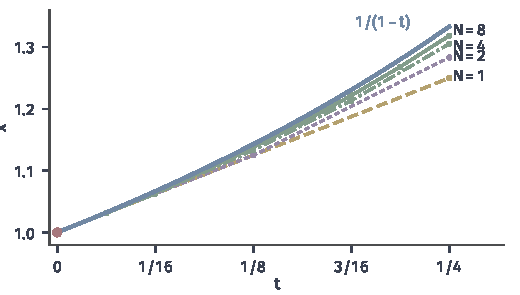
\includegraphics[width=88mm]{figures/06-differential-equations/01-ordinary-differential-equations/matplotlib/odeex-euler-refinement/figure.pdf}
  \caption{初值问题$\dot x=x^2$，$x(0)=1$在$[0,1/4]$上的Euler折线。蓝色粗线是真解$1/(1-t)$，其余折线的步数$N$分别为$1,2,4,8$，红点是初值。步数增加时折线向真解靠拢。}
  \label{fig:odeex-euler-refinement}
\end{BookInlineFigure}

这里的真解是预先知道的。对一般的连续右端，没有真解可作比较，也无从知道折线列是否收敛。我们手里只有折线本身的信息，要从中取出一条极限曲线，就要先把折线关在一个固定的范围内。

\paragraph{盒子与时间窗}
先选一个以初值为中心的盒子。取$a,b>0$足够小，记
\begin{equation}
 \bm{B}_b=\{\bm{x}\in\mathbb{R}^{n}:\lVert\bm{x}-\bm{x}_0\rVert_2\leq b\},\qquad
 \bm{Q}=[t_0-a,t_0+a]\times\bm{B}_b,
 \label{eq:odeex-box}
\end{equation}
使$\bm{Q}\subseteq\bm{D}$。$\bm{D}$是开集，这总能做到。$\bm{Q}$是紧集，连续函数$\lVert\bm{f}\rVert_2$在其上有最大值，取$M>0$使$\lVert\bm{f}\rVert_2\leq M$在$\bm{Q}$上成立。

$M$是盒子内箭头的最大速度。一条曲线只要还在盒子内，到初值的距离就至多以速率$M$增长，所以它被限制在以$(t_0,\bm{x}_0)$为顶点、斜率$\pm M$的锥内。它可能从盒子的上下壁离开，这要花至少$b/M$的时间；也可能走到盒子的左右壁，这要花时间$a$。于是在时间窗
\begin{equation}
 \delta=\min\Bigl\{a,\frac{b}{M}\Bigr\}
 \label{eq:odeex-peano-window}
\end{equation}
内，曲线不会离开盒子。

图~\ref{fig:odeex-existence-box}用前面的方程演示这一计算。取$b=1$，状态范围是$[0,2]$，其上$x^2\leq4$，所以$M=4$。图(a)中$a=1/2$，$\delta=\min\{1/2,1/4\}=1/4$，锥先碰到上壁。图(b)中$a=3/20$，$\delta=3/20$，锥先碰到右壁。真解实际能走到$t=1$，时间窗只是一个保守的保证。

\begin{BookInlineFigure}
  \centering
  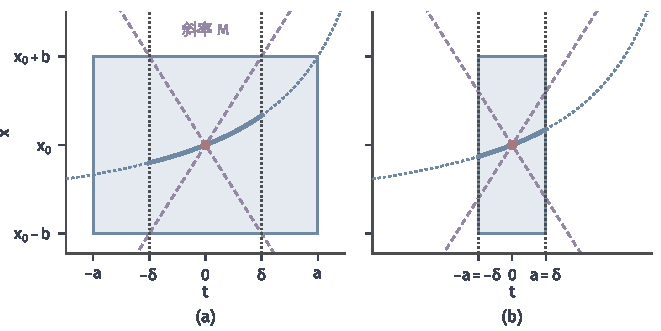
\includegraphics[width=112mm]{figures/06-differential-equations/01-ordinary-differential-equations/matplotlib/odeex-existence-box/figure.pdf}
  \caption{盒子与时间窗。浅蓝矩形是$\bm{Q}$，这里$x_0=1$，$b=1$，紫色虚线是斜率$\pm M=\pm4$的锥，蓝色粗线是真解在时间窗内的部分，蓝色点线是它在窗外的延续。(a)$a=1/2$，$\delta=b/M=1/4$，由状态范围决定。(b)$a=3/20$，$\delta=a$，由时间范围决定。}
  \label{fig:odeex-existence-box}
\end{BookInlineFigure}

\paragraph{Peano存在定理}
盒子内的折线有共同的速度上限，这件事足以让我们从折线列中抽出一条收敛的曲线。结论是下面的\term{Peano存在定理}（Peano existence theorem）。

\begin{theorem}[Peano存在定理]
\label{thm:odeex-peano}
设$\bm{D}\subseteq\mathbb{R}\times\mathbb{R}^{n}$是开集，$\bm{f}:\bm{D}\to\mathbb{R}^{n}$连续，$(t_0,\bm{x}_0)\in\bm{D}$。按式~\eqref{eq:odeex-box}取$\bm{Q}\subseteq\bm{D}$，取$M>0$使$\lVert\bm{f}\rVert_2\leq M$在$\bm{Q}$上成立，再按式~\eqref{eq:odeex-peano-window}确定$\delta$。则初值问题~\eqref{eq:odeex-ivp}在$[t_0-\delta,t_0+\delta]$上至少有一个经典解，解的取值都在$\bm{B}_b$中。
\end{theorem}

证明分三步：折线留在盒子内，折线列有一致收敛的子列，子列的极限满足积分方程。第一步用$\bm{f}$的有界性，第二步用有限维的紧性，第三步用$\bm{f}$的连续性。

\begin{proof}
先在$I^+=[t_0,t_0+\delta]$上构造解。对正整数$N$，取$h=\delta/N$，按式~\eqref{eq:odeex-euler-node}得到节点$\bm{x}^{(0)},\ldots,\bm{x}^{(N)}$，记相应的折线为$\bm{y}_N$，即对$t\in[t_k,t_{k+1}]$，
\[
 \bm{y}_N(t)=\bm{x}^{(k)}+(t-t_k)\,\bm{f}(t_k,\bm{x}^{(k)}).
\]

\emph{折线留在盒子内。}对$k$归纳证明$\lVert\bm{x}^{(k)}-\bm{x}_0\rVert_2\leq Mkh$。$k=0$时成立。若对$k<N$成立，则$Mkh\leq M\delta\leq b$，$(t_k,\bm{x}^{(k)})\in\bm{Q}$，所以$\lVert\bm{f}(t_k,\bm{x}^{(k)})\rVert_2\leq M$，于是
\[
 \lVert\bm{x}^{(k+1)}-\bm{x}_0\rVert_2\leq\lVert\bm{x}^{(k)}-\bm{x}_0\rVert_2+hM\leq M(k+1)h.
\]
因此所有节点都在球$\bm{B}_b$中。球是凸集，线段也在其中，折线的取值全在$\bm{B}_b$内，节点上的速度都不超过$M$。

\emph{抽取收敛子列。}折线每段的斜率范数不超过$M$，所以对$s,t\in I^+$，
\[
 \lVert\bm{y}_N(t)-\bm{y}_N(s)\rVert_2\leq M\lvert t-s\rvert.
\]
这说明$\{\bm{y}_N\}$的各分量等度连续，而它们又一致有界（取值在$\bm{B}_b$中）。紧区间上一致有界且等度连续的实函数族，由Arzelà--Ascoli判据在一致距离下相对紧，每个序列都有一致收敛的子列，可参考\BookChapterRef{chap:function-class-covers}{卷四第13章“函数类的有限覆盖”}。对$n$个分量依次抽取子列，得到$\bm{y}_{N_j}$一致收敛到连续曲线$\bm{x}:I^+\to\bm{B}_b$。

\emph{极限满足积分方程。}对$s\in[t_k,t_{k+1})$，记$\sigma_N(s)=t_k$，它是$s$所在网格段的左端点。折线分段线性，由其构造，
\[
 \bm{y}_N(t)=\bm{x}_0+\int_{t_0}^{t}\bm{f}\bigl(\sigma_N(s),\bm{y}_N(\sigma_N(s))\bigr)\,\mathrm{d}s.
\]
$\bm{f}$在紧集$\bm{Q}$上一致连续。任取$\varepsilon>0$，存在$\eta>0$，使$\bm{Q}$中两点的时间差与状态距离之和小于$\eta$时，$\bm{f}$值之差的范数小于$\varepsilon$。

比较被积函数在两点的取值：时间差是$s-\sigma_N(s)\leq h$，状态差由三角不等式与斜率上限满足
\[
 \lVert\bm{y}_N(\sigma_N(s))-\bm{x}(s)\rVert_2\leq Mh+\lVert\bm{y}_N-\bm{x}\rVert_{\infty},
\]
这里$\lVert\cdot\rVert_{\infty}$是$I^+$上的一致范数。沿子列$N=N_j$，$h\to0$，$\lVert\bm{y}_N-\bm{x}\rVert_{\infty}\to0$，所以当$j$足够大时，两点距离之和小于$\eta$，对所有$s$都有被积函数之差小于$\varepsilon$。

积分后得到，对$t\in I^+$，
\[
 \Bigl\lVert\int_{t_0}^{t}\bm{f}\bigl(\sigma_N(s),\bm{y}_N(\sigma_N(s))\bigr)\,\mathrm{d}s
 -\int_{t_0}^{t}\bm{f}(s,\bm{x}(s))\,\mathrm{d}s\Bigr\rVert_2\leq\varepsilon\delta.
\]
令$j\to\infty$，$\bm{x}$在$I^+$上满足积分方程~\eqref{eq:odeex-integral}。

\emph{向左延伸。}令$\tilde{\bm{x}}(s)=\bm{x}(2t_0-s)$，方程变成
\[
 \frac{\mathrm{d}\tilde{\bm{x}}}{\mathrm{d}s}=-\bm{f}(2t_0-s,\tilde{\bm{x}}),
\]
其右端满足同样的条件和同样的上界。对它应用前面的结论，得到$[t_0-\delta,t_0]$上的解。两段在$t_0$处都取$\bm{x}_0$，合起来在整个区间上满足式~\eqref{eq:odeex-integral}，因而是经典解。
\end{proof}

\paragraph{连续性在哪里起作用}
证明第三步用连续性把折线所用的箭头换成极限曲线上的箭头。若右端不连续，这一步会失败，解也可能真的不存在。取
\[
 f(x)=\begin{cases}-1,&x\geq0,\\ 1,&x<0,\end{cases}\qquad x(0)=0.
\]
箭头从两侧都指向$x=0$，图~\ref{fig:odeex-discontinuous-chatter}(a)中从$x=\pm1$出发的解都在$t=1$到达零线，到达之后就停在那里。

假设有解从$x(0)=0$出发。若解在某段时间内为正，这段时间的左端点处解为零，而解在段内以速度$-1$下降，不可能从$0$变成正数；同理解不能在某段时间内为负。于是解只能恒为零，而$\dot x=0$不等于$f(0)=-1$，矛盾。

Euler折线看到的是什么？在图~\ref{fig:odeex-discontinuous-chatter}(b)中，它在$0$与$-h$之间来回跳动，当$h\to0$时一致收敛到$x\equiv0$。折线列本身有极限，但折线所用的斜率在$\pm1$之间振荡，平均为$0$，而$f(0)=-1$。极限曲线不满足方程，正是因为第三步的“被积函数收敛”不成立。

\begin{BookInlineFigure}
  \centering
  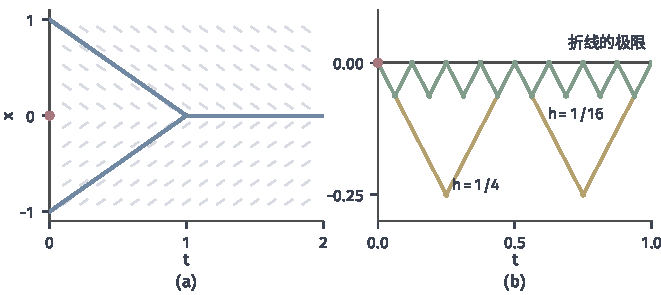
\includegraphics[width=112mm]{figures/06-differential-equations/01-ordinary-differential-equations/matplotlib/odeex-discontinuous-chatter/figure.pdf}
  \caption{右端不连续时存在性失败。$f(x)=-1$（$x\geq0$），$f(x)=1$（$x<0$）。(a)短线是方向场，蓝线是从$x=\pm1$出发的解，到$t=1$时汇入零线后停止延伸，红点是无解的初值$(0,0)$。(b)从红点出发的两条Euler折线，黄线$h=1/4$，绿线$h=1/16$，$h\to0$时一致趋于灰线$x\equiv0$，该极限不是解。}
  \label{fig:odeex-discontinuous-chatter}
\end{BookInlineFigure}

\paragraph{连续不保证唯一}
定理~\ref{thm:odeex-peano}说“至少一个”，这个说法不能加强。考虑
\begin{equation}
 \dot x=2\sqrt{\lvert x\rvert},\qquad x(0)=0.
 \label{eq:odeex-sqrt}
\end{equation}
右端处处连续。$x\equiv0$代入后两端都是零，成立。对$x=t^2$（$t\geq0$），左端$2t$，右端$2\sqrt{t^2}=2t$，也成立。

不止这两条。对每个$c\geq0$，定义
\[
 x_c(t)=\begin{cases}0,&t\leq c,\\(t-c)^2,&t>c.\end{cases}
\]
在$t>c$时验证与刚才相同，在$t=c$处左右导数都是$0$，等于右端的值，所以$x_c$是经典解。解可以在零线上停留任意长的时间，然后在任意时刻起飞。图~\ref{fig:odeex-sqrt-funnel}画出了这束解，它们从同一个红点出发，初值完全相同，将来却不同。

\begin{BookInlineFigure}
  \centering
  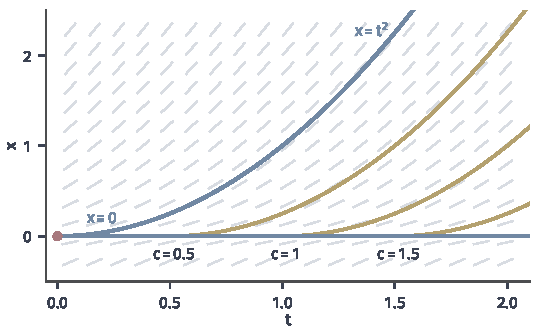
\includegraphics[width=92mm]{figures/06-differential-equations/01-ordinary-differential-equations/matplotlib/odeex-sqrt-funnel/figure.pdf}
  \caption{初值问题~\eqref{eq:odeex-sqrt}的多个解。短线是方向场，红点是初值$(0,0)$。蓝线是$x\equiv0$与$x=t^2$，黄线是在$t=c$时离开零线的解$x_c$，$c=0.5,1,1.5$。任意$c\geq0$都给出一条解。}
  \label{fig:odeex-sqrt-funnel}
\end{BookInlineFigure}

为什么连续性不足以挑出一条解？$x$接近$0$时，箭头斜率$2\sqrt{\lvert x\rvert}$相对于$\lvert x\rvert$大得不成比例：比值$2/\sqrt{\lvert x\rvert}$趋于无穷。于是离开零线一点点就有足够的速度继续远离，离开零线并不需要一个有限的“推力”。

多解还解释了为什么证明中要抽子列。考虑方程
\[
 \dot x=2\operatorname{sgn}(x)\sqrt{\lvert x\rvert},\qquad x(0)=0,
\]
它同样有解$x\equiv0$和$x=\pm t^2$。若折线的初值恰好是$0$，它恒为零；但若初值带一个微小的扰动$x^{(0)}=(-1)^N/N^2$，比如计算时的舍入，$N$为偶数和奇数时折线会走向不同的解。

取$N$为偶数，步长$h=\delta/N$，其中$\delta=1$。令$s_k=\sqrt{x^{(k)}}$，由式~\eqref{eq:odeex-euler-node}，
\[
 s_{k+1}^2=s_k^2+2hs_k.
\]
当$s_k\geq h/4$时，$(s_k+h/2)^2=s_k^2+hs_k+h^2/4\leq s_k^2+2hs_k$，所以$s_{k+1}\geq s_k+h/2$。而$s_0=1/N=h$，于是对所有$k$，
\[
 x^{(k)}\geq\bigl(s_0+kh/2\bigr)^2\geq\Bigl(\frac{t_k}{2}\Bigr)^2.
\]

奇数$N$的折线是偶数情形的镜像。所以偶数列的极限至少是$t^2/4$，奇数列的极限至多是$-t^2/4$，整列折线没有极限，如图~\ref{fig:odeex-odd-sqrt-euler}所示。紧性只给出“有收敛的子列”，不同子列可以收敛到不同的解。

\begin{BookInlineFigure}
  \centering
  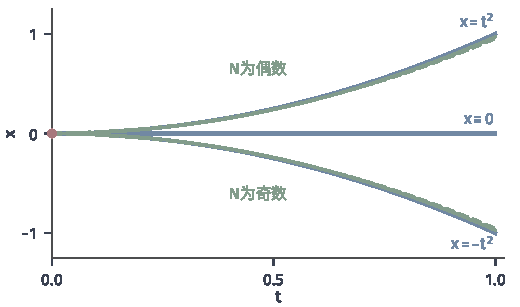
\includegraphics[width=88mm]{figures/06-differential-equations/01-ordinary-differential-equations/matplotlib/odeex-odd-sqrt-euler/figure.pdf}
  \caption{$\dot x=2\operatorname{sgn}(x)\sqrt{\lvert x\rvert}$的Euler折线，初值$x^{(0)}=(-1)^N/N^2$，步长$1/N$。绿色虚线$N=20,21$，绿色实线$N=80,81$，蓝线是从$(0,0)$出发的三条解。偶数$N$贴近$t^2$，奇数$N$贴近$-t^2$，整列不收敛。}
  \label{fig:odeex-odd-sqrt-euler}
\end{BookInlineFigure}

\paragraph{紧性只属于有限维}
证明的第二步用了“一致有界且等度连续的曲线族相对紧”。它的前提是每个时刻的取值落在一个紧集中，而$\mathbb{R}^{n}$的闭球恰好是紧的。在无限维空间中闭球不紧，这一步不能照搬，结论也确实会失败。

设$c_0$是收敛到零的实数列$\bm{x}=(x_1,x_2,\ldots)$组成的空间，范数取各坐标绝对值的上确界，记为$\lVert\bm{x}\rVert_{\infty}$，它是完备的。定义$\bm{f}:c_0\to c_0$，
\[
 \bigl(\bm{f}(\bm{x})\bigr)_n=2\sqrt{\lvert x_n\rvert}+\frac{1}{n+1},\qquad n\geq1.
\]
第一项随$n\to\infty$趋于零，第二项也是，所以$\bm{f}(\bm{x})\in c_0$。对实数$a,b$，有
\[
 \lvert\sqrt{\lvert a\rvert}-\sqrt{\lvert b\rvert}\rvert\leq\sqrt{\lvert a-b\rvert}.
\]
逐坐标使用它，得到
\[
 \lVert\bm{f}(\bm{x})-\bm{f}(\bm{y})\rVert_{\infty}\leq2\sqrt{\lVert\bm{x}-\bm{y}\rVert_{\infty}},
\]
所以$\bm{f}$连续。

假设$\bm{x}(t)$是$[0,\delta)$上取值于$c_0$的解，$\bm{x}(0)=\bm{0}$。在范数下可微蕴含每个坐标可微，所以每个坐标满足$\dot x_n=2\sqrt{\lvert x_n\rvert}+1/(n+1)>0$。于是$x_n(t)>0$对$t>0$成立，并且
\[
 \frac{\mathrm{d}}{\mathrm{d}t}\sqrt{x_n}=\frac{\dot x_n}{2\sqrt{x_n}}\geq1.
\]
从$s>0$积分到$t$，再令$s\downarrow0$，得到$\sqrt{x_n(t)}\geq t$，即对所有$n$，
\[
 x_n(t)\geq t^2.
\]
每个坐标都不低于同一个正数，这与$\bm{x}(t)\in c_0$矛盾。因此这个连续方程在$c_0$中没有解。

图~\ref{fig:odeex-c0-coordinates}算出了各坐标的实际取值。右端的序列在$t=0$时衰减，解的坐标却被$t^2$托住，在任何$t>0$时都不再衰减到零。$\bm{f}$的连续性和局部有界性都在，只是缺了紧性。

\begin{BookInlineFigure}
  \centering
  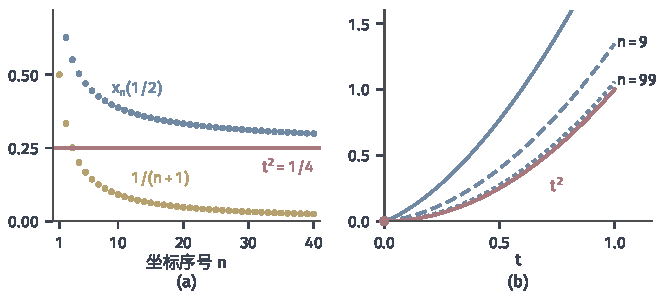
\includegraphics[width=112mm]{figures/06-differential-equations/01-ordinary-differential-equations/matplotlib/odeex-c0-coordinates/figure.pdf}
  \caption{$c_0$中无解方程的坐标。各坐标单独满足$\dot x_n=2\sqrt{x_n}+1/(n+1)$，$x_n(0)=0$，由数值积分算出。(a)$t=1/2$时的取值，蓝点$x_n(1/2)$都在红线$t^2=1/4$之上，黄点$1/(n+1)$是右端在$t=0$的序列。(b)蓝线为$n=1,9,99$时的$x_n(t)$，都在红线$t^2$之上，$n$增大时趋于$t^2$而不趋于$0$。}
  \label{fig:odeex-c0-coordinates}
\end{BookInlineFigure}

\section{唯一性}
\label{sec:odeex-uniqueness}

漏斗状的多解出现在$\dot x=2\sqrt{\lvert x\rvert}$的零线上，那里右端随状态变化得太快。反过来想，什么样的右端能阻止两条解分开？设$\bm{u},\bm{v}$是同一初值的两条解，它们的差的变化率是$\bm{f}(t,\bm{u})-\bm{f}(t,\bm{v})$。若这个量能用差本身来控制，两条解一开始重合，就没有东西推动它们分开。

\paragraph{状态方向的Lipschitz条件}
把“右端的变化能用状态差控制”写成条件。下面只比较同一时刻的两个状态，时间方向没有光滑性要求。

\begin{definition}[状态方向的局部Lipschitz条件]
\label{def:odeex-local-lipschitz}
设$\bm{D}\subseteq\mathbb{R}\times\mathbb{R}^{n}$开，$\bm{f}:\bm{D}\to\mathbb{R}^{n}$。若对每点$(t_\ast,\bm{x}_\ast)\in\bm{D}$，存在它的邻域$\bm{U}\subseteq\bm{D}$和常数$L\geq0$，使对$\bm{U}$中所有同一时刻的两点$(t,\bm{x}),(t,\bm{y})$都有
\begin{equation}
 \lVert\bm{f}(t,\bm{x})-\bm{f}(t,\bm{y})\rVert_2\leq L\lVert\bm{x}-\bm{y}\rVert_2,
 \label{eq:odeex-lipschitz}
\end{equation}
就称$\bm{f}$在状态方向\term{局部Lipschitz连续}（locally Lipschitz continuous），且该性质对时间局部一致。
\end{definition}

定义里的“局部一致”指同一个$L$对邻域内所有时刻都有效。几何上，固定时刻后，以$(\bm{x},\bm{f}(t,\bm{x}))$为顶点、斜率$L$的双锥把邻域内其余部分的图像都关在里面。图~\ref{fig:odeex-lipschitz-secants}比较三个函数。

\begin{BookInlineFigure}
  \centering
  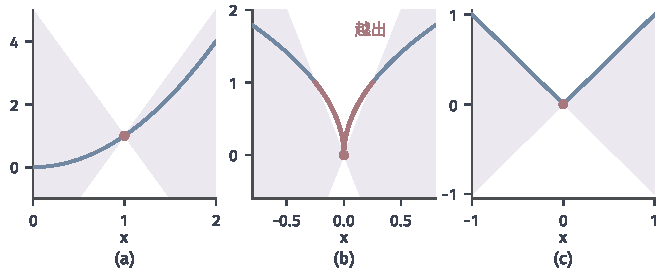
\includegraphics[width=112mm]{figures/06-differential-equations/01-ordinary-differential-equations/matplotlib/odeex-lipschitz-secants/figure.pdf}
  \caption{状态方向的Lipschitz条件。蓝线是函数图像，红点是基点，紫色区域是斜率$L$的双锥。(a)$x^2$在$[0,2]$上，基点$x=1$，$L=4$，图像在双锥内。(b)$2\sqrt{\lvert x\rvert}$，基点$x=0$，$L=4$，红色部分越出双锥；增大$L$只能缩小越出的范围，不能消除。(c)$\lvert x\rvert$，$L=1$，在基点不可微，图像仍在双锥内。}
  \label{fig:odeex-lipschitz-secants}
\end{BookInlineFigure}

图(a)的$x^2$在$[0,2]$上满足条件：
\[
 \lvert x^2-y^2\rvert=\lvert x+y\rvert\,\lvert x-y\rvert\leq4\lvert x-y\rvert.
\]
它在整条实轴上没有统一的$L$，这正是“局部”二字的用处。图(b)的$2\sqrt{\lvert x\rvert}$在原点不满足条件，这与多解的出现位置一致。图(c)说明Lipschitz条件比可微弱，折角并不妨碍它。

验证条件最常用的办法是求导。若$\partial_{\bm{x}}\bm{f}$存在且在$\bm{D}$上连续，在一个球形邻域内连接$\bm{x},\bm{y}$的线段上积分，得到
\[
 \bm{f}(t,\bm{x})-\bm{f}(t,\bm{y})
 =\int_0^1\partial_{\bm{x}}\bm{f}\bigl(t,\bm{y}+\theta(\bm{x}-\bm{y})\bigr)(\bm{x}-\bm{y})\,\mathrm{d}\theta.
\]
在紧邻域上取$L$为$\lVert\partial_{\bm{x}}\bm{f}\rVert_2$的最大值，就得到式~\eqref{eq:odeex-lipschitz}。

\paragraph{主要思想：积分方程是不动点问题}
积分方程~\eqref{eq:odeex-integral}把解刻画成一个自洽条件。给定一条曲线$\bm{u}$，沿它读出箭头，积分出一条新曲线，记为
\begin{equation}
 (\mathcal{T}\bm{u})(t)=\bm{x}_0+\int_{t_0}^{t}\bm{f}(s,\bm{u}(s))\,\mathrm{d}s.
 \label{eq:odeex-picard-map}
\end{equation}
解就是$\mathcal{T}$的不动点：把它代入，得到的还是它自己。把曲线看成无限维向量（每个时刻是一个坐标），$\mathcal{T}$是这个向量空间上的一个映射，初值问题就成了解方程$\bm{x}=\mathcal{T}\bm{x}$。

解这个方程最朴素的办法是反复代入。从常值曲线$\bm{x}^{(0)}(t)\equiv\bm{x}_0$出发，令
\begin{equation}
 \bm{x}^{(k+1)}=\mathcal{T}\bm{x}^{(k)},\quad k=0,1,\ldots,
 \label{eq:odeex-picard-iteration}
\end{equation}
这一列曲线称为\term{Picard迭代}（Picard iteration）。本节中上标$(k)$表示迭代次数，每个$\bm{x}^{(k)}$是一整条曲线。

\begin{example}[指数函数的Picard迭代]
\label{ex:odeex-picard-exp}
取$\dot x=x$，$x(0)=1$，此时$(\mathcal{T}u)(t)=1+\int_0^tu(s)\,\mathrm{d}s$。前几步分别是
\[
 x^{(0)}=1,\quad x^{(1)}=1+t,\quad x^{(2)}=1+t+\frac{t^2}{2}.
\]

设$x^{(k)}(t)=\sum_{j=0}^{k}t^j/j!$，代入式~\eqref{eq:odeex-picard-map}，逐项积分得到
\[
 x^{(k+1)}(t)=1+\sum_{j=0}^{k}\frac{t^{j+1}}{(j+1)!}=\sum_{j=0}^{k+1}\frac{t^j}{j!}.
\]
所以Picard迭代就是指数级数的部分和。在$[0,1]$上，余项满足
\[
 \lvert\mathrm{e}^t-x^{(k)}(t)\rvert\leq\frac{\mathrm{e}}{(k+1)!}.
\]
\end{example}

图~\ref{fig:odeex-picard-exp}显示，每迭代一次，曲线多贴合真解一段。对这个例子，迭代既不是在时间方向上推进，也不是逐点修正，而是每次把整条曲线替换一遍。

\begin{BookInlineFigure}
  \centering
  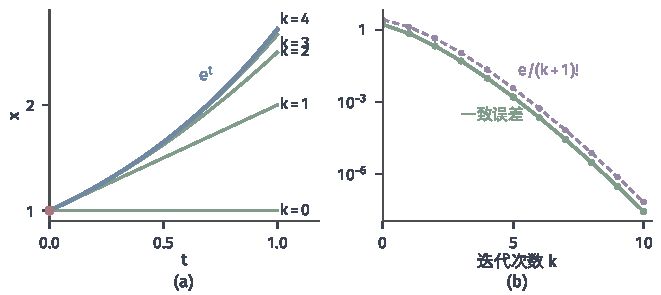
\includegraphics[width=112mm]{figures/06-differential-equations/01-ordinary-differential-equations/matplotlib/odeex-picard-exp/figure.pdf}
  \caption{$\dot x=x$，$x(0)=1$的Picard迭代。(a)绿线是$x^{(0)},\ldots,x^{(4)}$，蓝线是真解$\mathrm{e}^t$，红点是初值。(b)$[0,1]$上的一致误差（绿线）与上界$\mathrm{e}/(k+1)!$（紫色虚线），纵轴为对数坐标；衰减比任何几何级数都快。}
  \label{fig:odeex-picard-exp}
\end{BookInlineFigure}

\paragraph{为什么要缩短时间窗}
要保证迭代一般都收敛，自然想到压缩映射定理：完备度量空间上的压缩映射有唯一不动点，迭代从任何初值出发都收敛到它，可参考\BookChapterRef{chap:metric-space-maps}{卷四第3章“度量空间上的映射”}，那里也证明了区间上的连续函数在一致距离下完备。下面估计$\mathcal{T}$对曲线距离的作用。

设$\bm{u},\bm{v}$是两条曲线，$(s,\bm{u}(s))$和$(s,\bm{v}(s))$都在Lipschitz条件成立的盒子内。对$\lvert t-t_0\rvert\leq\delta$，由积分的范数不等式与式~\eqref{eq:odeex-lipschitz}，
\[
 \lVert(\mathcal{T}\bm{u})(t)-(\mathcal{T}\bm{v})(t)\rVert_2
 \leq\Bigl\lvert\int_{t_0}^{t}L\lVert\bm{u}(s)-\bm{v}(s)\rVert_2\,\mathrm{d}s\Bigr\rvert
 \leq L\delta\sup_{s}\lVert\bm{u}(s)-\bm{v}(s)\rVert_2.
\]

$\mathcal{T}$对距离的放大倍数至多是$L\delta$。积分把两条曲线的差沿时间累积，累积的时间越短，差就越小；$\delta$足够小时，这个映射就是压缩的。

图~\ref{fig:odeex-integral-smoothing}对$\dot x=x^2$，$x(0)=1$演示了这一点。两条任意选取的曲线在$[-1/8,1/8]$上一致距离约为$1.31$，经$\mathcal{T}$作用后，距离约为$0.125$，比值约$0.095$，小于这里的压缩常数$1/2$。

\begin{BookInlineFigure}
  \centering
  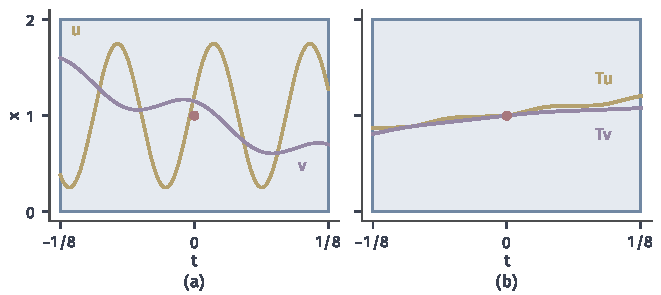
\includegraphics[width=112mm]{figures/06-differential-equations/01-ordinary-differential-equations/matplotlib/odeex-integral-smoothing/figure.pdf}
  \caption{积分映射缩小曲线距离。方程为$\dot x=x^2$，$x(0)=1$，浅蓝矩形是$\lvert t\rvert\leq1/8$、$\lvert x-1\rvert\leq1$的盒子。(a)盒内两条任取的曲线$u$（黄）和$v$（紫）。(b)它们的像$\mathcal{T}u$和$\mathcal{T}v$，都过红色初值点，振荡被积分抹平，一致距离由约$1.31$降为约$0.125$。}
  \label{fig:odeex-integral-smoothing}
\end{BookInlineFigure}

只缩短时间窗还不够，$\mathcal{T}$要把所选的曲线集合映回自身，否则迭代中途可能离开盒子，式~\eqref{eq:odeex-lipschitz}就不能再用。第~\ref{sec:odeex-local-existence}节的锥形估计恰好处理这件事。把这两个要求放在一起，就是\term{Picard--Lindelöf定理}（Picard--Lindelöf theorem）。

\begin{theorem}[Picard--Lindelöf定理]
\label{thm:odeex-picard-lindelof}
设$\bm{f}:\bm{D}\to\mathbb{R}^{n}$，$\bm{Q}=[t_0-a,t_0+a]\times\bm{B}_b\subseteq\bm{D}$，$\bm{f}$在$\bm{Q}$上连续，并存在$M,L>0$，使$\lVert\bm{f}\rVert_2\leq M$与式~\eqref{eq:odeex-lipschitz}在$\bm{Q}$上成立。令
\begin{equation}
 \delta=\min\Bigl\{a,\frac{b}{M},\frac{1}{2L}\Bigr\},\qquad I_\delta=[t_0-\delta,t_0+\delta].
 \label{eq:odeex-picard-window}
\end{equation}
则：
\begin{enumerate}
 \item 初值问题~\eqref{eq:odeex-ivp}在$I_\delta$上有经典解$\bm{x}$，其取值都在$\bm{B}_b$中；
 \item 若$I'\subseteq I_\delta$是含$t_0$的区间，$\bm{y}$是$I'$上的任一经典解，则$\bm{y}=\bm{x}$在$I'$上成立；
 \item Picard迭代~\eqref{eq:odeex-picard-iteration}在$I_\delta$上一致收敛到$\bm{x}$，且对$k\geq1$，
 \begin{equation}
 \lVert\bm{x}^{(k)}-\bm{x}\rVert_{\infty}\leq2^{1-k}\lVert\bm{x}^{(1)}-\bm{x}^{(0)}\rVert_{\infty},\qquad
 \lVert\bm{x}^{(k)}-\bm{x}\rVert_{\infty}\leq\lVert\bm{x}^{(k)}-\bm{x}^{(k-1)}\rVert_{\infty}.
 \label{eq:odeex-picard-error}
 \end{equation}
\end{enumerate}
\end{theorem}

\begin{proof}
\emph{选取空间。}记$\lVert\bm{y}\rVert_{\infty}$为$\lVert\bm{y}(t)\rVert_2$在$I_\delta$上的最大值，$C(I_\delta;\mathbb{R}^{n})$在这个范数下完备。令
\[
 \mathcal{X}=\bigl\{\bm{u}\in C(I_\delta;\mathbb{R}^{n}):\lVert\bm{u}(t)-\bm{x}_0\rVert_2\leq b,\ \forall t\in I_\delta\bigr\}.
\]
$\mathcal{X}$是闭集，一致收敛保持逐点的不等式，所以$\mathcal{X}$在一致距离下是完备度量空间；它含常值曲线$\bm{x}_0$，非空。

\emph{映回自身。}设$\bm{u}\in\mathcal{X}$。由$\delta\leq a$，点$(s,\bm{u}(s))$对$s\in I_\delta$都在$\bm{Q}$中，$s\mapsto\bm{f}(s,\bm{u}(s))$连续，积分有定义，$\mathcal{T}\bm{u}$连续。由$\delta\leq b/M$，
\[
 \lVert(\mathcal{T}\bm{u})(t)-\bm{x}_0\rVert_2
 \leq\Bigl\lvert\int_{t_0}^{t}\lVert\bm{f}(s,\bm{u}(s))\rVert_2\,\mathrm{d}s\Bigr\rvert
 \leq M\lvert t-t_0\rvert\leq b.
\]
所以$\mathcal{T}\bm{u}\in\mathcal{X}$。

\emph{压缩。}对$\bm{u},\bm{v}\in\mathcal{X}$，点$(s,\bm{u}(s)),(s,\bm{v}(s))$都在$\bm{Q}$中，前面的估计给出
\[
 \lVert\mathcal{T}\bm{u}-\mathcal{T}\bm{v}\rVert_{\infty}\leq L\delta\lVert\bm{u}-\bm{v}\rVert_{\infty}\leq\frac12\lVert\bm{u}-\bm{v}\rVert_{\infty}.
\]

\emph{不动点。}由压缩映射定理，$\mathcal{T}$在$\mathcal{X}$中有唯一不动点$\bm{x}$，Picard迭代从$\bm{x}^{(0)}\equiv\bm{x}_0\in\mathcal{X}$出发一致收敛到$\bm{x}$，其先验误差界和后验误差界取压缩常数$q=1/2$，就是式~\eqref{eq:odeex-picard-error}。不动点满足积分方程~\eqref{eq:odeex-integral}，因而是经典解。结论1和结论3得证。

\emph{任何解都留在盒内。}设$\bm{y}$是$I'$上的解。只看$t\geq t_0$的一侧，另一侧相同。令$t^\ast$为使$\bm{y}$在$[t_0,t]\cap I'$上取值于$\bm{B}_b$的$t$的上确界。在$[t_0,t^\ast)\cap I'$上点$(s,\bm{y}(s))$在$\bm{Q}$中，所以$\lVert\bm{y}(t)-\bm{x}_0\rVert_2\leq M(t-t_0)$在其上成立。

若$t^\ast$小于$I'$的右端点，则$t^\ast<t_0+\delta$，由连续性，
\[
 \lVert\bm{y}(t^\ast)-\bm{x}_0\rVert_2\leq M(t^\ast-t_0)<M\delta\leq b.
\]
这是严格不等式，$\bm{y}$在$t^\ast$之后一小段时间内还在球内，与上确界的定义矛盾。所以$\bm{y}$在$I'$上始终留在$\bm{B}_b$中。

\emph{唯一性。}两条解$\bm{x},\bm{y}$在$I'$上都留在盒内，都满足积分方程。记$e=\sup_{t\in I'}\lVert\bm{x}(t)-\bm{y}(t)\rVert_2$，它不超过$2b$，是有限数。相减并用式~\eqref{eq:odeex-lipschitz}，
\[
 \lVert\bm{x}(t)-\bm{y}(t)\rVert_2\leq L\delta\,e\leq\frac12e.
\]
对$t\in I'$取上确界，得$e\leq e/2$，即$e=0$，结论2得证。
\end{proof}

定理中各条件分工明确。$\bm{Q}\subseteq\bm{D}$让方程有定义；$\delta\leq b/M$让$\mathcal{T}$不把曲线带出盒子；$\delta\leq1/(2L)$让距离缩小；连续性让积分有定义，并使不动点是经典解。完备性保证迭代的柯西列有极限，这里用不到任何紧性。

\paragraph{计算过程}
Picard迭代的每一步都要计算一条曲线的积分，下面用$\dot x=x^2$，$x(0)=1$手算到第三轮，完整走一遍。取$a=1/2$，$b=1$，由图~\ref{fig:odeex-lipschitz-secants}(a)的计算，$M=4$，$L=4$，所以
\[
 \delta=\min\Bigl\{\frac12,\frac14,\frac18\Bigr\}=\frac18,\qquad q=L\delta=\frac12.
\]

\needspace{6\baselineskip}
\paragraph{变量}
\begin{itemize}
 \item $x^{(k)}$：第$k$轮的曲线，定义在$I_\delta=[-1/8,1/8]$上，例中都是多项式；
 \item $\Delta^{(k)}$：相邻两轮的一致距离$\lVert x^{(k)}-x^{(k-1)}\rVert_{\infty}$，用于后验误差界；
 \item $\varepsilon$：给定的误差容许值，例中取$2\times10^{-3}$。
\end{itemize}

\needspace{6\baselineskip}
\paragraph{初始化}
令$\bm{x}^{(0)}(t)\equiv\bm{x}_0$。例中$x^{(0)}=1$。

\needspace{6\baselineskip}
\paragraph{每轮更新}
对$k=0,1,\ldots$，依次执行：
\begin{enumerate}
 \item 由式~\eqref{eq:odeex-picard-iteration}，把$\bm{x}^{(k)}$代入右端并积分，得到$\bm{x}^{(k+1)}$。

 例中第一轮的被积函数是$1$，所以
 \[
 x^{(1)}(t)=1+t.
 \]
 第二轮对$(1+s)^2$积分，得到
 \[
 x^{(2)}(t)=1+t+t^2+\frac{t^3}{3}.
 \]
 第三轮对$(1+s+s^2+s^3/3)^2$积分，得到
 \[
 x^{(3)}(t)=1+t+t^2+t^3+\frac23t^4+\frac13t^5+\frac19t^6+\frac{1}{63}t^7.
 \]
 \item 计算$\Delta^{(k+1)}$。例中相邻两轮的差都在$t=1/8$处取到最大模，于是
 \[
 \Delta^{(1)}=\frac18,\quad \Delta^{(2)}\approx1.63\times10^{-2},\quad \Delta^{(3)}\approx1.48\times10^{-3}.
 \]
 \item 若后验误差界$q\Delta^{(k+1)}/(1-q)$不超过$\varepsilon$，就停止，否则继续。由式~\eqref{eq:odeex-picard-error}，$q=1/2$时这个界就是$\Delta^{(k+1)}$。

 例中$\Delta^{(2)}>\varepsilon$，第二轮后继续；$\Delta^{(3)}\leq\varepsilon$，第三轮后停止。
\end{enumerate}

最终得到$x^{(3)}$，它在$[-1/8,1/8]$上与真解的误差被保证不超过$1.48\times10^{-3}$。实际误差约为$1.06\times10^{-4}$，比界小一个数量级。

图~\ref{fig:odeex-picard-square}(a)显示迭代在时间窗内很快贴合真解，窗外贴合得较慢，越靠近真解的奇点$t=1$差得越远。图(b)比较实际误差和先验界$2^{1-k}\cdot1/8$，先验界用的是全局的$q=1/2$，实际误差衰减得快得多。

\begin{BookInlineFigure}
  \centering
  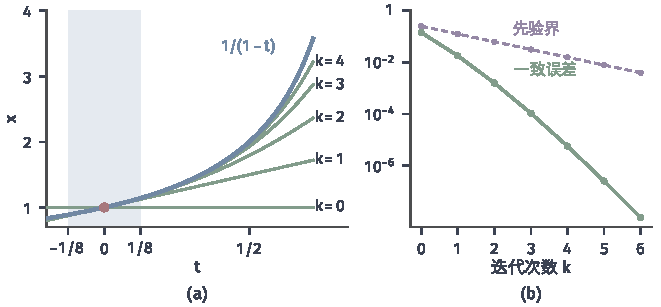
\includegraphics[width=112mm]{figures/06-differential-equations/01-ordinary-differential-equations/matplotlib/odeex-picard-square/figure.pdf}
  \caption{$\dot x=x^2$，$x(0)=1$的Picard迭代。(a)绿线是$x^{(0)},\ldots,x^{(4)}$，蓝线是真解，浅蓝带是时间窗$[-1/8,1/8]$。(b)时间窗上的一致误差（绿线）与先验界$2^{1-k}\cdot\tfrac18$（紫色虚线），纵轴为对数坐标。}
  \label{fig:odeex-picard-square}
\end{BookInlineFigure}

\paragraph{时间窗不必缩到$1/(2L)$}
定理中的$1/(2L)$是为了让$\mathcal{T}$在一步之内就成为压缩映射。例~\ref{ex:odeex-picard-exp}在$[0,1]$上有$L\delta=1$，不是压缩，迭代却收敛得比几何级数还快。原因是误差要累积多次才会放大，而累积的时间区域越来越窄。

设$\delta'=\min\{a,b/M\}$，定义域换成$I_{\delta'}$。前面“映回自身”的论证只用了$\delta'\leq a$与$\delta'\leq b/M$，所以$\mathcal{T}$仍把相应的$\mathcal{X}$映回自身，迭代都有定义。下面对$k\geq0$归纳证明，对$t\in I_{\delta'}$，
\begin{equation}
 \lVert\bm{x}^{(k+1)}(t)-\bm{x}^{(k)}(t)\rVert_2\leq\frac{ML^{k}\lvert t-t_0\rvert^{k+1}}{(k+1)!}.
 \label{eq:odeex-picard-factorial}
\end{equation}

$k=0$时，左端是$\bm{f}(s,\bm{x}_0)$积分的范数，被积函数的范数不超过$M$，所以不超过$M\lvert t-t_0\rvert$。设$k-1$时成立，对$t\geq t_0$，由式~\eqref{eq:odeex-lipschitz}，
\[
 \lVert\bm{x}^{(k+1)}(t)-\bm{x}^{(k)}(t)\rVert_2
 \leq L\int_{t_0}^{t}\frac{ML^{k-1}(s-t_0)^{k}}{k!}\,\mathrm{d}s
 =\frac{ML^{k}(t-t_0)^{k+1}}{(k+1)!}.
\]
$t<t_0$的情形相同。

式~\eqref{eq:odeex-picard-factorial}的右端对$k$求和收敛，和不超过$M(\mathrm{e}^{L\delta'}-1)/L$，所以$\bm{x}^{(k)}$一致收敛，其极限是$\mathcal{T}$的不动点。两个不动点的差用同样的归纳，得到对任意$k$，
\[
 \lVert\bm{u}(t)-\bm{v}(t)\rVert_2\leq2b\,\frac{(L\lvert t-t_0\rvert)^{k}}{k!},
\]
令$k\to\infty$，差为零。任何解都留在盒内的论证也只用到$\delta'\leq b/M$。因此解在整个$I_{\delta'}$上存在且唯一，时间窗的长度由$a$和$b/M$决定，不受$L$限制；$L$只影响收敛的快慢。

\paragraph{Lipschitz条件只是充分条件}
定理给出的是唯一性的充分条件，并不必要。考虑方向相反的方程
\[
 \dot x=-2\operatorname{sgn}(x)\sqrt{\lvert x\rvert}.
\]
它在原点同样不满足Lipschitz条件。但右端关于$x$单调不增，两条解$u,v$之差满足
\[
 \frac{\mathrm{d}}{\mathrm{d}t}(u-v)^2=2(u-v)\bigl(f(u)-f(v)\bigr)\leq0.
\]
所以差只会减小，初值相同的两条解在$t$增大的方向上不会分开，向前唯一。

图~\ref{fig:odeex-one-sided-merge}显示了这个方程的解：从$x_0$出发的解是$\operatorname{sgn}(x_0)(\sqrt{\lvert x_0\rvert}-t)^2$，在$t=\sqrt{\lvert x_0\rvert}$到达零线后停在那里，不同的解在有限时间内合并。把时间倒过来，方程变成式~\eqref{eq:odeex-sqrt}的奇函数版本，从零线出发可以有多条解，所以向后不唯一。这里的唯一性来自单调性，与Lipschitz条件无关。

\begin{BookInlineFigure}
  \centering
  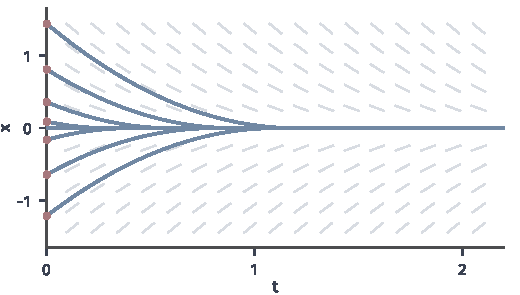
\includegraphics[width=88mm]{figures/06-differential-equations/01-ordinary-differential-equations/matplotlib/odeex-one-sided-merge/figure.pdf}
  \caption{$\dot x=-2\operatorname{sgn}(x)\sqrt{\lvert x\rvert}$的解。短线是方向场，红点是不同的初值，蓝线是相应的解，在有限时间内汇入零线。向前的解由初值确定，向后从零线出发则有多个可能。}
  \label{fig:odeex-one-sided-merge}
\end{BookInlineFigure}

\paragraph{Lipschitz常数要对时间局部一致}
定义~\ref{def:odeex-local-lipschitz}要求$L$在邻域内对时间一致。如果每个时刻各有一个常数，但常数随时间无界，唯一性也会失败。令$\operatorname{clip}(x;0,t^2)$表示把$x$截断到$[0,t^2]$，定义
\begin{equation}
 f(t,x)=\begin{cases}\dfrac{2}{t}\operatorname{clip}(x;0,t^2),&t>0,\\0,&t\leq0.\end{cases}
 \label{eq:odeex-clip}
\end{equation}

由$0\leq\operatorname{clip}\leq t^2$，有$\lvert f(t,x)\rvert\leq2t$，所以$f$在$t=0$处连续，从而在$\mathbb{R}^{2}$上连续。固定$t>0$，$f$关于$x$是Lipschitz的，常数为$2/t$；固定$t\leq0$，$f$恒为零。每个时刻单独看都满足条件，但常数$2/t$在$t\to0$时无界。

对每个$c\in[0,1]$，曲线$x=ct^2$满足$0\leq x\leq t^2$，右端等于$2ct$，恰是它的导数。所以从$x(0)=0$出发有无穷多条解，如图~\ref{fig:odeex-time-lipschitz}所示。两条解的差以$2/t$的相对速率增长，这个速率在$t=0$附近的积分发散，足以从零差产生非零差。

\begin{BookInlineFigure}
  \centering
  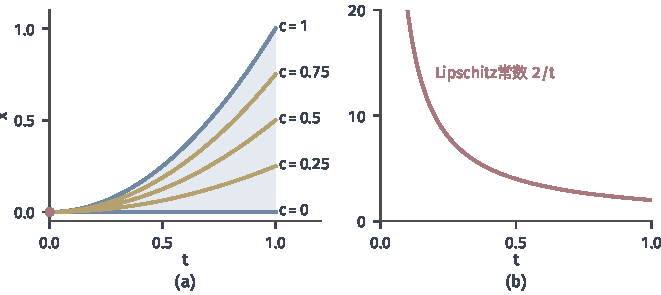
\includegraphics[width=112mm]{figures/06-differential-equations/01-ordinary-differential-equations/matplotlib/odeex-time-lipschitz/figure.pdf}
  \caption{Lipschitz常数对时间不一致导致多解。(a)方程~\eqref{eq:odeex-clip}的解$x=ct^2$，浅蓝区域$0\leq x\leq t^2$内，$c$取$0,0.25,0.5,0.75,1$，都从红点出发。(b)固定时刻的Lipschitz常数$2/t$，在$t\to0$时无界。}
  \label{fig:odeex-time-lipschitz}
\end{BookInlineFigure}

\paragraph{紧性与完备性}
Peano和Picard两条路线用的工具不同，结论的强弱也不同，表~\ref{tab:odeex-peano-picard}把它们放在一起。

\begin{BookInlineTable}
  \centering
  \caption{两条存在性路线的对比}
  \label{tab:odeex-peano-picard}
  \begin{tabular}{lll}
    \toprule
     & Peano路线 & Picard路线 \\
    \midrule
    右端条件 & 连续 & 连续，状态方向Lipschitz \\
    逼近对象 & Euler折线 & Picard迭代 \\
    收敛来源 & 紧性，只有子列 & 完备性，整列收敛 \\
    结论 & 至少一个解 & 恰有一个解，有误差界 \\
    无限维空间 & 可能无解 & 证明不变，结论成立 \\
    \bottomrule
  \end{tabular}
\end{BookInlineTable}

最后一行值得注意。Picard路线只用到空间的完备性和范数不等式，状态空间换成任何完备的赋范空间，证明的步骤不变，只需假设盒子上$\bm{f}$有界且满足Lipschitz条件。第~\ref{sec:odeex-local-existence}节$c_0$上的反例恰好不满足Lipschitz条件。

\section{最大延拓}
\label{sec:odeex-maximal}

Picard--Lindelöf定理只保证一小段时间。到达时间窗的尽头后，把终点当作新的初值再解一段，解就能接着往前走。这个过程能继续多久，走不下去时发生了什么？本节在定义~\ref{def:odeex-local-lipschitz}的条件下回答。以下总设$\bm{D}\subseteq\mathbb{R}\times\mathbb{R}^{n}$开，$\bm{f}:\bm{D}\to\mathbb{R}^{n}$连续，并在状态方向局部Lipschitz连续，该性质对时间局部一致。

\paragraph{相容的局部解}
拼接之前要确认，两段局部解在重叠处不会打架。局部唯一性只在一个小窗内成立，下面的引理把它传播到任意长的公共区间上，办法是看两条解重合的时刻组成的集合。

\begin{lemma}[公共区间上的唯一性]
\label{lem:odeex-common-uniqueness}
设$\bm{x}_1,\bm{x}_2$分别是区间$I_1,I_2$上的经典解，$I_1\cap I_2$含$t_0$，且$\bm{x}_1(t_0)=\bm{x}_2(t_0)$。则$\bm{x}_1=\bm{x}_2$在$I_1\cap I_2$上成立。
\end{lemma}

\begin{proof}
记$I=I_1\cap I_2$，它是区间。令$S=\{t\in I:\bm{x}_1(t)=\bm{x}_2(t)\}$，它含$t_0$。两条解连续，所以$S$在$I$中闭。

下面证明$S$在$I$中开。任取$t^\ast\in S$，记$\bm{x}^\ast=\bm{x}_1(t^\ast)$。在$(t^\ast,\bm{x}^\ast)$的邻域内，由定义~\ref{def:odeex-local-lipschitz}，可以取一个盒子和常数$M,L$，使定理~\ref{thm:odeex-picard-lindelof}的条件成立，得到时间窗$[t^\ast-\delta,t^\ast+\delta]$。

$\bm{x}_1,\bm{x}_2$在区间$I\cap[t^\ast-\delta,t^\ast+\delta]$上都是以$(t^\ast,\bm{x}^\ast)$为初值的经典解，由定理的结论2，它们都等于窗上的唯一解，所以这段区间包含在$S$中。

$I$是连通的，$S$是它的非空开闭子集，于是$S=I$。
\end{proof}

图~\ref{fig:odeex-gluing}(a)画的是两段解的重叠，引理保证重叠部分是同一条曲线。图(b)是证明的核心：若两条解有“第一次分开”的时刻$t^\ast$，在该时刻的状态附近局部唯一性就被破坏了，所以这样的时刻不存在。

\begin{BookInlineFigure}
  \centering
  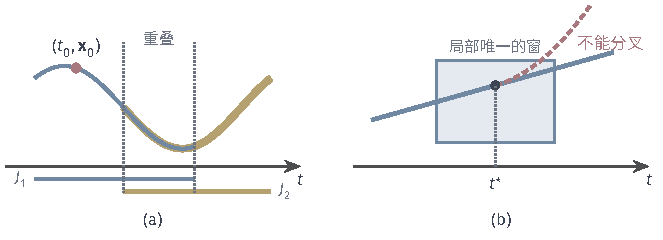
\includegraphics[width=112mm]{figures/06-differential-equations/01-ordinary-differential-equations/tikz/odeex-gluing/figure.pdf}
  \caption{局部解的相容性。(a)区间$J_1$（蓝）与$J_2$（黄）上的两段解经过同一初值，在重叠的时间段内是同一条曲线，并起来是更长区间上的解。(b)若两条解在$t^\ast$之后分开（红色虚线），在$(t^\ast,\bm{x}(t^\ast))$的小窗（浅蓝矩形）内就有两个解，与局部唯一性矛盾。}
  \label{fig:odeex-gluing}
\end{BookInlineFigure}

\paragraph{最大解}
有了相容性，就可以把所有局部解并起来。设$\bm{x}$是区间$I$上的解，$\tilde{\bm{x}}$是区间$\tilde I\supsetneq I$上的解，且$\tilde{\bm{x}}$在$I$上等于$\bm{x}$，就称$\tilde{\bm{x}}$是$\bm{x}$的一个\term{解的延拓}（continuation of a solution）。不能再延拓的解称为\term{最大解}（maximal solution），它的定义区间称为\term{最大存在区间}（maximal interval of existence）。

\begin{theorem}[最大解]
\label{thm:odeex-maximal}
对每点$(t_0,\bm{x}_0)\in\bm{D}$，初值问题~\eqref{eq:odeex-ivp}存在唯一的最大解$\bm{x}:I_{\max}\to\mathbb{R}^{n}$，其中$I_{\max}=(\omega_-,\omega_+)$是含$t_0$的开区间，$-\infty\leq\omega_-<\omega_+\leq+\infty$。该初值问题的每个解都是最大解在某个子区间上的限制。
\end{theorem}

\begin{proof}
设$\{(I_\alpha,\bm{x}_\alpha)\}$是该初值问题的全部解，由定理~\ref{thm:odeex-picard-lindelof}，这个族非空。各$I_\alpha$都含$t_0$，所以$I_{\max}=\bigcup_\alpha I_\alpha$是区间。对$t\in I_{\max}$，取含$t$的$I_\alpha$，令$\bm{x}(t)=\bm{x}_\alpha(t)$，由引理~\ref{lem:odeex-common-uniqueness}，这个值与$\alpha$的选取无关。

$t_0$到$t$的闭区间含于$I_\alpha$，在其上$\bm{x}=\bm{x}_\alpha$，所以$\bm{x}$在$t$处满足积分方程~\eqref{eq:odeex-integral}。这对每个$t\in I_{\max}$成立，且被积函数连续，因此$\bm{x}$是$I_{\max}$上的经典解。

$\bm{x}$不能延拓，否则延拓后的解属于上述族，其定义区间含于$I_{\max}$。每个解都是$\bm{x}$的限制，这由构造得到，唯一性随之成立。

最后证明$I_{\max}$是开区间。若右端点$\omega_+$属于$I_{\max}$，则$(\omega_+,\bm{x}(\omega_+))\in\bm{D}$，从这一点解局部初值问题，得到$[\omega_+-\delta,\omega_++\delta]$上的解$\bm{z}$。由引理~\ref{lem:odeex-common-uniqueness}，$\bm{z}$在左半段与$\bm{x}$相同。

令曲线在$I_{\max}$上等于$\bm{x}$、在$[\omega_+,\omega_++\delta]$上等于$\bm{z}$，它在$\omega_+$处连续，并在整个区间上满足积分方程，是比$\bm{x}$更长的解，矛盾。左端点同理。
\end{proof}

\paragraph{窗口为什么会越来越短}
以$\dot x=x^2$，$x(0)=1$为例，$\bm{D}=\mathbb{R}^{2}$，最大解是$1/(1-t)$，$I_{\max}=(-\infty,1)$。把“重启”过程具体算一遍，看看解为什么过不了$t=1$。

设已走到$(t_k,x_k)$，取半径$b=x_k$的盒子，$a$取得足够大，此时状态范围是$[0,2x_k]$，$M=4x_k^2$，第~\ref{sec:odeex-uniqueness}节的时间窗$\delta'=\min\{a,b/M\}$给出
\[
 \delta_k=\frac{x_k}{4x_k^2}=\frac{1}{4x_k}=\frac{1-t_k}{4}.
\]
最后一步用了$x_k=1/(1-t_k)$。于是下一个重启时刻满足$1-t_{k+1}=\tfrac34(1-t_k)$，从$t_0=0$开始，
\[
 t_k=1-\Bigl(\frac34\Bigr)^{k},\qquad x_k=\Bigl(\frac43\Bigr)^{k},\qquad\delta_k=\frac14\Bigl(\frac34\Bigr)^{k}.
\]

前几个重启时刻是
\[
 t_1=0.25,\quad t_2=0.4375,\quad t_3\approx0.5781.
\]
窗口长度成等比下降，总和恰好是$1$，无限次重启也越不过$t=1$，如图~\ref{fig:odeex-continuation-windows}。窗口变短的原因是状态增大，箭头变快，同样高度的盒子能撑的时间变短。

\begin{BookInlineFigure}
  \centering
  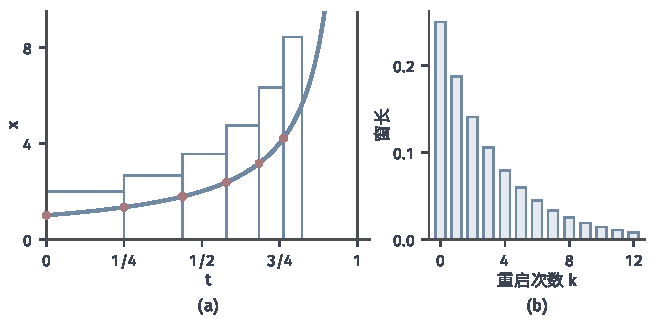
\includegraphics[width=112mm]{figures/06-differential-equations/01-ordinary-differential-equations/matplotlib/odeex-continuation-windows/figure.pdf}
  \caption{沿$\dot x=x^2$重启局部定理。(a)蓝线是真解，红点是重启点$(t_k,x_k)$，矩形是每次重启所用的时间窗$\delta_k$与状态范围$[0,2x_k]$，灰色竖线是$t=1$。(b)窗长$\delta_k=\tfrac14(3/4)^k$随重启次数按等比衰减，总和为$1$。}
  \label{fig:odeex-continuation-windows}
\end{BookInlineFigure}

这个例子提示了一般规律。时间窗只依赖盒子内的$M$和$L$。如果解始终留在一个固定的紧集内，$M,L$有共同的上界，窗口有一个不随重启变化的正下限，重启有限次就能越过任何有限时刻。所以解走不下去，只能是因为它没有留在任何紧集内。

\paragraph{紧集上的统一时间窗}
把这个想法写严格，需要两个引理：局部Lipschitz常数在紧集上可以取成统一的，局部定理的时间窗在紧集上也可以取成统一的。

\begin{lemma}[紧集上的统一Lipschitz常数]
\label{lem:odeex-compact-lipschitz}
设$\bm{K}\subseteq\bm{D}$是紧集。则存在常数$L$，使式~\eqref{eq:odeex-lipschitz}对$\bm{K}$中所有同一时刻的两点$(t,\bm{x}),(t,\bm{y})$成立。
\end{lemma}

\begin{proof}
设$M=\max_{\bm{K}}\lVert\bm{f}\rVert_2$。假设结论不成立，则对每个正整数$j$，存在$\bm{K}$中同一时刻的两点$(t_j,\bm{x}_j),(t_j,\bm{y}_j)$，使
\[
 \lVert\bm{f}(t_j,\bm{x}_j)-\bm{f}(t_j,\bm{y}_j)\rVert_2>j\lVert\bm{x}_j-\bm{y}_j\rVert_2.
\]
左端不超过$2M$，所以$\lVert\bm{x}_j-\bm{y}_j\rVert_2<2M/j\to0$。

由紧性，取子列使$(t_j,\bm{x}_j)$收敛到某点$(t_\ast,\bm{x}_\ast)\in\bm{K}$，此时$(t_j,\bm{y}_j)$也收敛到同一点。该点有定义~\ref{def:odeex-local-lipschitz}中的邻域和常数$L_\ast$，当$j$足够大时两点都在这个邻域内，不等号的左端不超过$L_\ast\lVert\bm{x}_j-\bm{y}_j\rVert_2$，再取$j>L_\ast$即得矛盾。
\end{proof}

\begin{lemma}[紧集上的统一时间窗]
\label{lem:odeex-uniform-window}
设$\bm{K}\subseteq\bm{D}$是紧集。则存在$\delta_{\bm{K}}>0$，使对每点$(s,\bm{\xi})\in\bm{K}$，以$(s,\bm{\xi})$为初值的问题在$[s-\delta_{\bm{K}},s+\delta_{\bm{K}}]$上有解。
\end{lemma}

\begin{proof}
若$\bm{D}$不是全空间，紧集$\bm{K}$到闭集$\bm{D}^{\mathrm{c}}$的距离大于零，取正数$\rho$小于这个距离的一半，否则取$\rho=1$。令
\[
 \bm{K}'=\bigl\{(t,\bm{x}):\exists(s,\bm{\xi})\in\bm{K},\ \lvert t-s\rvert\leq\rho/2,\ \lVert\bm{x}-\bm{\xi}\rVert_2\leq\rho/2\bigr\}.
\]
$\bm{K}'$是$\bm{K}$与一个紧盒子的和，因而紧，并且$\bm{K}'\subseteq\bm{D}$。

在$\bm{K}'$上取$M>0$为$\lVert\bm{f}\rVert_2$的上界，由引理~\ref{lem:odeex-compact-lipschitz}取$L>0$。对$\bm{K}$中任一点，$a=b=\rho/2$的盒子都含于$\bm{K}'$，定理~\ref{thm:odeex-picard-lindelof}给出共同的时间窗
\[
 \delta_{\bm{K}}=\min\Bigl\{\frac{\rho}{2},\frac{\rho}{2M},\frac{1}{2L}\Bigr\}.
\]
这就是所要的常数。
\end{proof}

\paragraph{离开每个紧集}
现在可以把“走不下去”说清楚。

\begin{theorem}[最大解离开紧集]
\label{thm:odeex-escape}
设$\bm{x}:(\omega_-,\omega_+)\to\mathbb{R}^{n}$是最大解。对每个紧集$\bm{K}\subseteq\bm{D}$，存在$t_{\bm{K}}\in(\omega_-,\omega_+)$，使当$t\in(t_{\bm{K}},\omega_+)$时，都有$(t,\bm{x}(t))\notin\bm{K}$。左端点$\omega_-$有对称的结论。
\end{theorem}

\begin{proof}
反设存在紧集$\bm{K}$和$t_j\uparrow\omega_+$，使$(t_j,\bm{x}(t_j))\in\bm{K}$。$\bm{K}$在时间方向有界，所以$\omega_+<+\infty$。

取引理~\ref{lem:odeex-uniform-window}中的$\delta_{\bm{K}}$，再取$j$使$t_j+\delta_{\bm{K}}>\omega_+$。以$(t_j,\bm{x}(t_j))$为初值的解$\bm{z}$在$[t_j-\delta_{\bm{K}},t_j+\delta_{\bm{K}}]$上存在，由引理~\ref{lem:odeex-common-uniqueness}，它在公共区间上与$\bm{x}$相同。

$\bm{z}$的定义区间越过了$\omega_+$，把$\bm{x}$与$\bm{z}$并起来就得到比最大解更长的解，矛盾。
\end{proof}

注意结论是“最终离开并且不再回来”，比“离开过”强。证明正是靠这一点：只要解在$\omega_+$附近回到$\bm{K}$一次，时间窗就能把它带过$\omega_+$。

\paragraph{两种障碍}
最常见的定义域是乘积形式$\bm{D}=J\times\bm{\Omega}$，其中$J$是右端给定的开时间区间，$\bm{\Omega}\subseteq\mathbb{R}^{n}$是开集。设$\omega_+<\sup J$，即解在右端还有定义的时候就停止了。对$\bm{\Omega}$的每个紧子集$\bm{C}$，$[t_0,\omega_+]\times\bm{C}$是$\bm{D}$的紧子集，由定理~\ref{thm:odeex-escape}，$\bm{x}(t)$在$\omega_+$之前最终离开$\bm{C}$。

特别地，状态空间是整个$\mathbb{R}^{n}$时，取$\bm{C}$为半径任意大的闭球，得到：若$\omega_+<\sup J$，则
\begin{equation}
 \lim_{t\uparrow\omega_+}\lVert\bm{x}(t)\rVert_2=+\infty.
 \label{eq:odeex-blowup-alternative}
\end{equation}
这就是有限时间爆炸。对一般的$\bm{\Omega}$，紧子集可以取成“离$\bm{\Omega}$的边界不太近且范数不太大”的集合，解要离开它们，要么范数趋于无穷，要么趋近$\bm{\Omega}$的边界，也可能在两者之间来回。

图~\ref{fig:odeex-exit-obstacles}给出三种典型情况，三个方程的右端都在各自定义域内满足本节的条件，$\omega_+=1$。

\begin{BookInlineFigure}
  \centering
  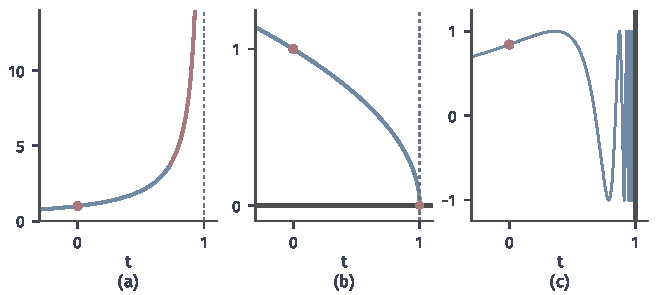
\includegraphics[width=112mm]{figures/06-differential-equations/01-ordinary-differential-equations/matplotlib/odeex-exit-obstacles/figure.pdf}
  \caption{最大解在$\omega_+=1$处结束的三种情形，红点是初值，灰色粗线是定义域的边界。(a)$\dot x=x^2$，$\bm{D}=\mathbb{R}^{2}$，状态趋于无穷（红色部分）。(b)$\dot x=-1/(2x)$，$\bm{D}=\mathbb{R}\times(0,\infty)$，解$\sqrt{1-t}$有界，趋近状态边界$x=0$。(c)$\bm{D}=(-\infty,1)\times\mathbb{R}$，解$\sin(1/(1-t))$有界且没有极限，时间到达定义域的边界$t=1$。}
  \label{fig:odeex-exit-obstacles}
\end{BookInlineFigure}

图(a)是状态无界的障碍：$\bm{\Omega}=\mathbb{R}$，解按式~\eqref{eq:odeex-blowup-alternative}趋于无穷。图(b)是逼近定义域边界的障碍：对$\dot x=-1/(2x)$，$x(0)=1$，由$(x^2)'=-1$得到$x=\sqrt{1-t}$，它在$t\uparrow1$时有界地趋于$0$，而$0$不在$\bm{\Omega}=(0,\infty)$中，右端在那里无定义，解不能再走。

图(c)是时间区间本身的端点：方程$\dot x=\cos\bigl(1/(1-t)\bigr)/(1-t)^2$，$x(0)=\sin1$的解是$\sin\bigl(1/(1-t)\bigr)$。此时$\omega_+=\sup J=1$，不属于式~\eqref{eq:odeex-blowup-alternative}的情形，定理~\ref{thm:odeex-escape}仍然成立，因为$(t,\bm{x}(t))$的时间分量趋向$\bm{D}$的边界。解有界但在$t\uparrow1$时没有极限，可见“离开紧集”不等于“收敛到某个边界点”。

\section{全局存在}
\label{sec:odeex-global}

状态空间是$\mathbb{R}^{n}$时，最大解只有一种走不到时间区间尽头的方式：范数趋于无穷。于是只要能预先证明解在任何有限时间段上有界，爆炸就被排除了，解会一直延续到右端给定的整个时间区间。这样的解称为\term{全局解}（global solution）。

\paragraph{爆炸快慢由增长速度决定}
先看标量自治方程，算出爆炸发生的时刻。设$f$在$[x_0,\infty)$上连续且为正，局部Lipschitz，解单调上升。由$\mathrm{d}t=\mathrm{d}x/f(x)$，走到无穷所需的时间是
\begin{equation}
 T=\int_{x_0}^{\infty}\frac{\mathrm{d}x}{f(x)}.
 \label{eq:odeex-blowup-time}
\end{equation}
这个积分有限时，解在$T$时刻爆炸；无穷时，解不爆炸。状态越大，箭头越快，走过单位状态所用的时间$1/f(x)$越短，这些时间加起来可能有限。

取$f(x)=x^p$，$x_0=1$。$p>1$时
\[
 T=\int_1^\infty x^{-p}\,\mathrm{d}x=\frac{1}{p-1},
\]
$p=2$时$T=1$，与前面的结果一致。$p=1$时积分发散，解是$\mathrm{e}^t$，增长虽快，但在有限时间内走不到无穷。线性增长正是这个分界线。图~\ref{fig:odeex-blowup-integral}(a)比较了$1/x^2$和$1/x$的尾部面积，图(b)比较了相应的解。

\begin{BookInlineFigure}
  \centering
  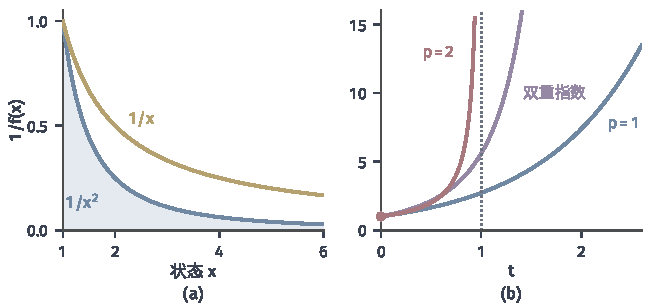
\includegraphics[width=112mm]{figures/06-differential-equations/01-ordinary-differential-equations/matplotlib/odeex-blowup-integral/figure.pdf}
  \caption{增长速度与有限时间爆炸。(a)走过单位状态的用时$1/f(x)$：蓝线$1/x^2$的尾部面积（浅蓝）有限，等于$1$；黄线$1/x$的尾部面积无穷。(b)初值都为$x(0)=1$的解：红线$\dot x=x^2$在$t=1$爆炸，蓝线$\dot x=x$是$\mathrm{e}^t$，紫线$\dot x=(1+x)\ln(1+x)$是$2^{\mathrm{e}^t}-1$，增长比线性快但不爆炸。}
  \label{fig:odeex-blowup-integral}
\end{BookInlineFigure}

\paragraph{至多线性增长}
线性增长是分界线，这一观察对向量方程仍然有用，只要把$\lVert\bm{f}\rVert_2$用状态范数的一次函数控制住。系数可以随时间变化，甚至只要局部可积。

\begin{theorem}[线性增长下的全局存在]
\label{thm:odeex-global}
设$J\subseteq\mathbb{R}$是开区间，$\bm{f}:J\times\mathbb{R}^{n}\to\mathbb{R}^{n}$连续，在状态方向局部Lipschitz连续且对时间局部一致。若存在$J$上局部可积的非负函数$\alpha,\beta$，使对所有$t\in J$，$\bm{x}\in\mathbb{R}^{n}$，
\begin{equation}
 \lVert\bm{f}(t,\bm{x})\rVert_2\leq\alpha(t)\lVert\bm{x}\rVert_2+\beta(t),
 \label{eq:odeex-linear-growth}
\end{equation}
则对每个$(t_0,\bm{x}_0)\in J\times\mathbb{R}^{n}$，最大解定义在整个$J$上，并且对$t\in J$，
\begin{equation}
 \lVert\bm{x}(t)\rVert_2\leq\Bigl(\lVert\bm{x}_0\rVert_2+\Bigl\lvert\int_{t_0}^{t}\beta\Bigr\rvert\Bigr)\exp\Bigl\lvert\int_{t_0}^{t}\alpha\Bigr\rvert.
 \label{eq:odeex-global-bound}
\end{equation}
\end{theorem}

满足式~\eqref{eq:odeex-linear-growth}的右端称为\term{至多线性增长}（at most linear growth）。证明分两步：先证明界~\eqref{eq:odeex-global-bound}，再用它排除爆炸。

\begin{proof}
设$\bm{x}$是最大解，定义在$(\omega_-,\omega_+)$上。先看$t\geq t_0$的一侧。取$T\in[t_0,\omega_+)$，记$u(t)=\lVert\bm{x}(t)\rVert_2$，它是$[t_0,T]$上的连续函数。由积分方程~\eqref{eq:odeex-integral}和式~\eqref{eq:odeex-linear-growth}，对$t\in[t_0,T]$，
\[
 u(t)\leq\lVert\bm{x}_0\rVert_2+\int_{t_0}^{t}\bigl(\alpha(s)u(s)+\beta(s)\bigr)\,\mathrm{d}s\leq B+\int_{t_0}^{t}\alpha(s)u(s)\,\mathrm{d}s,
\]
其中$B=\lVert\bm{x}_0\rVert_2+\int_{t_0}^{T}\beta$。

把右端记作$v(t)$，它在$[t_0,T]$上绝对连续，几乎处处有$\dot v=\alpha u\leq\alpha v$。令$A(t)=\int_{t_0}^t\alpha$，$A$也绝对连续。绝对连续函数的乘积仍绝对连续，于是几乎处处有
\[
 \frac{\mathrm{d}}{\mathrm{d}t}\bigl(v\,\mathrm{e}^{-A}\bigr)=(\dot v-\alpha v)\,\mathrm{e}^{-A}\leq0.
\]
绝对连续函数可由导数积分恢复，所以$v\,\mathrm{e}^{-A}$单调不增，由此
\[
 v(T)\leq v(t_0)\,\mathrm{e}^{A(T)}=B\,\mathrm{e}^{A(T)}.
\]
这里用到的绝对连续函数的性质，可参考\BookChapterRef{chap:integration}{卷四第6章“积分”}。由$u(T)\leq v(T)$，式~\eqref{eq:odeex-global-bound}在$t=T$处成立。

设$\omega_+<\sup J$。此时$[t_0,\omega_+]$是$J$的紧子集，$\alpha,\beta$在其上可积，所以式~\eqref{eq:odeex-global-bound}的右端对$T<\omega_+$有一个与$T$无关的上界。这与式~\eqref{eq:odeex-blowup-alternative}矛盾，于是$\omega_+=\sup J$。

$t\leq t_0$的一侧，令$\tilde{\bm{x}}(s)=\bm{x}(2t_0-s)$，它满足右端为$-\bm{f}(2t_0-s,\cdot)$的方程，增长条件的系数换成$\alpha(2t_0-s),\beta(2t_0-s)$，应用前面的结论即可。
\end{proof}

条件各有分工。式~\eqref{eq:odeex-linear-growth}是全局条件，要求对所有状态成立，正是它阻止了爆炸；Lipschitz条件只是局部的，它负责唯一性和最大解的存在，不参与防止爆炸。$\alpha,\beta$在紧时间段上可积，$\exp\int\alpha$才是有限数。

\paragraph{几个例子}
\begin{example}[线性系统]
\label{ex:odeex-linear-global}
设$\bm{A}(t)$和$\bm{g}(t)$在开区间$J$上连续，$\bm{f}(t,\bm{x})=\bm{A}(t)\bm{x}+\bm{g}(t)$。在紧时间段上$\lVert\bm{A}(t)\rVert_2$有界，
\[
 \lVert\bm{f}(t,\bm{x})-\bm{f}(t,\bm{y})\rVert_2\leq\lVert\bm{A}(t)\rVert_2\lVert\bm{x}-\bm{y}\rVert_2,
\]
满足局部Lipschitz条件。增长条件取$\alpha=\lVert\bm{A}(t)\rVert_2$，$\beta=\lVert\bm{g}(t)\rVert_2$，因此每个初值问题的解都定义在整个$J$上，这正是第~\ref{chap:linear-differential-systems}章的传播公式成立的范围。
\end{example}

\begin{example}[单摆]
\label{ex:odeex-pendulum-global}
单摆方程$\ddot x=-\sin x$写成状态$(x,v)$的系统，右端$\bm{f}(x,v)=(v,-\sin x)$是非线性的。由$\lvert\sin x\rvert\leq\lvert x\rvert$，
\[
 \lVert\bm{f}(x,v)\rVert_2=\sqrt{v^2+\sin^2x}\leq\lVert(x,v)\rVert_2.
\]
取$\alpha=1$，$\beta=0$，单摆的解对所有$t\in\mathbb{R}$存在，并满足
\[
 \lVert(x,v)(t)\rVert_2\leq\lVert(x_0,v_0)\rVert_2\,\mathrm{e}^{\lvert t\rvert}.
\]
\end{example}

\begin{example}[界与真解的比较]
\label{ex:odeex-barrier}
取$\dot x=\sqrt{1+x^2}$，$x(0)=0$，真解是$\sinh t$。由$\sqrt{1+x^2}\leq1+\lvert x\rvert$，可取$\alpha=\beta=1$，式~\eqref{eq:odeex-global-bound}给出，对$t\geq0$，
\[
 \lvert x(t)\rvert\leq t\,\mathrm{e}^{t}.
\]
在$t=1$处，界约为$2.718$，真解约为$1.175$。
\end{example}

图~\ref{fig:odeex-linear-growth-barrier}把这个界和真解画在一起，并与右端只多了平方项的$\dot x=1+x^2$对照。界比真解松得多，但它对每个有限的$t$都是有限数，这已足够排除爆炸；$\dot x=1+x^2$的解$\tan t$不满足线性增长条件，在$t=\pi/2$爆炸。

\begin{BookInlineFigure}
  \centering
  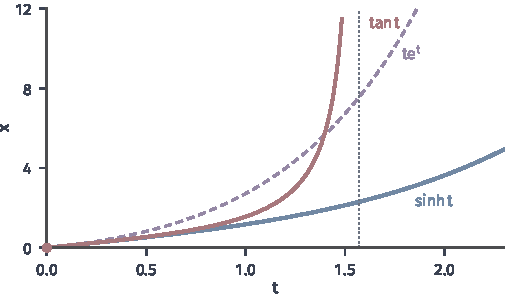
\includegraphics[width=88mm]{figures/06-differential-equations/01-ordinary-differential-equations/matplotlib/odeex-linear-growth-barrier/figure.pdf}
  \caption{线性增长下的上界。蓝线是$\dot x=\sqrt{1+x^2}$的解$\sinh t$，紫色虚线是由式~\eqref{eq:odeex-global-bound}得到的界$t\mathrm{e}^t$，红线是$\dot x=1+x^2$的解$\tan t$，在点线$t=\pi/2$处爆炸。初值都是$x(0)=0$。}
  \label{fig:odeex-linear-growth-barrier}
\end{BookInlineFigure}

\paragraph{条件的边界}
线性增长是充分条件，并不必要。前面图~\ref{fig:odeex-blowup-integral}(b)中的$\dot x=(1+x)\ln(1+x)$增长比线性快，令$y=\ln(1+x)$，方程化为$\dot y=y$，于是$x=2^{\mathrm{e}^t}-1$对所有$t$存在；由式~\eqref{eq:odeex-blowup-time}，这相当于$\int^{\infty}\mathrm{d}x/\bigl((1+x)\ln(1+x)\bigr)$发散。

符号也起作用。$\dot x=-x^3$的增长是三次的，但它把状态往零拉，解
\[
 x(t)=\frac{x_0}{\sqrt{1+2x_0^2t}}
\]
对所有$t\geq0$存在；向后走时，它在$t=-1/(2x_0^2)$爆炸。线性增长条件不看方向，所以它同时保证了两个时间方向的存在。

\paragraph{全局存在不是长期稳定}
定理~\ref{thm:odeex-global}只说解在每个有限时刻都有定义，不说解保持有界。$\dot x=x$的解$\mathrm{e}^t$全局存在，并趋于无穷；式~\eqref{eq:odeex-global-bound}的右端也随$t$增长。解的长期去向、是否靠近平衡点，要用另外的结构和条件来研究，可参考\BookChapterRef{chap:dynamical-systems-long-term}{卷九第1章“动力系统与轨迹的长期行为”}。

增长条件也不提供唯一性。式~\eqref{eq:odeex-sqrt}的右端满足$2\sqrt{\lvert x\rvert}\leq1+\lvert x\rvert$，是至多线性增长的，前面写出的解$x_c$对所有$t\geq0$都有定义，却有无穷多条。全局性与唯一性由不同的条件负责。

\section{时间可测的方程}
\label{sec:odeex-measurable}

前面的结论都要求右端对时间连续，但外部输入经常不连续。电路开关闭合、暖气切换功率时，输入在某些时刻跳变；更一般的输入可能只是一个可积函数。第~\ref{chap:ordinary-differential-equations}章已经看到，这类方程的解在跳变处有折角，不处处可微，要用积分方程来确定。对这样的右端，解的存在、唯一和延拓分别需要什么条件？

\paragraph{一个切换输入}
取$\dot x=-x+g(t)$，$x(0)=0$，其中$g(t)=1$（$0\leq t<1$），$g(t)=0$（$t\geq1$）。在$[0,1]$上解得
\[
 x(t)=1-\mathrm{e}^{-t},
\]
到$t=1$时$x(1)=1-\mathrm{e}^{-1}\approx0.632$。之后从这个值开始按齐次方程衰减，
\[
 x(t)=(1-\mathrm{e}^{-1})\,\mathrm{e}^{-(t-1)},\qquad t\geq1.
\]

两段在$t=1$处连续，但左导数是$\mathrm{e}^{-1}\approx0.368$，右导数是$-(1-\mathrm{e}^{-1})\approx-0.632$，如图~\ref{fig:odeex-measurable-switch}(b)。曲线处处满足积分方程，只在$t=1$这一点没有导数。

输入还可以无界。图~\ref{fig:odeex-measurable-switch}(c)的$\dot x=t^{-1/2}$，$x(0)=0$，在$t=0$处右端没有有限值，积分却收敛，解是$x=2\sqrt{t}$，在起点的切线是竖直的。把输入换成$1/t$就不行了：$\int_0^t\mathrm{d}s/s$发散，从$x(0)=0$出发的解不存在。可见起作用的不是有界性，而是右端在时间上可积。

\begin{BookInlineFigure}
  \centering
  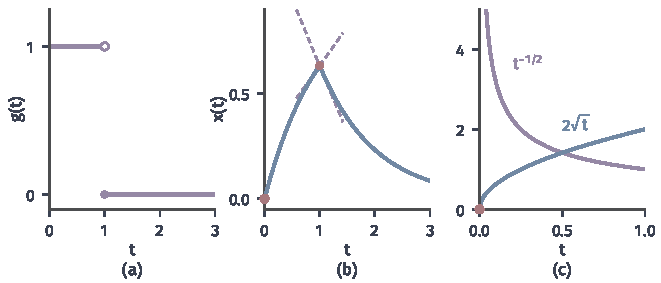
\includegraphics[width=112mm]{figures/06-differential-equations/01-ordinary-differential-equations/matplotlib/odeex-measurable-switch/figure.pdf}
  \caption{时间可测的右端。(a)切换输入$g$（紫线）。(b)$\dot x=-x+g(t)$，$x(0)=0$的解（蓝线），在$t=1$有折角，紫色虚线是左右两侧的切线。(c)无界但可积的输入$t^{-1/2}$（紫线）和解$2\sqrt{t}$（蓝线）。}
  \label{fig:odeex-measurable-switch}
\end{BookInlineFigure}

\paragraph{条件与解的定义}
把上面的观察写成条件。下面$J$是区间，$\bm{\Omega}\subseteq\mathbb{R}^{n}$是开集。

\begin{definition}[Carathéodory条件]
\label{def:odeex-caratheodory}
称$\bm{f}:J\times\bm{\Omega}\to\mathbb{R}^{n}$满足\term{Carathéodory条件}（Carathéodory conditions），是指：
\begin{enumerate}
 \item 对每个$\bm{x}\in\bm{\Omega}$，$t\mapsto\bm{f}(t,\bm{x})$是Lebesgue可测的；
 \item 对几乎每个$t\in J$，$\bm{x}\mapsto\bm{f}(t,\bm{x})$连续；
 \item 对每个紧区间$J'\subseteq J$和紧集$\bm{C}\subseteq\bm{\Omega}$，存在$m\in L^1(J')$，使对几乎每个$t\in J'$和所有$\bm{x}\in\bm{C}$，都有
 \begin{equation}
 \lVert\bm{f}(t,\bm{x})\rVert_2\leq m(t).
 \label{eq:odeex-caratheodory-bound}
 \end{equation}
\end{enumerate}
\end{definition}

第三条是局部可积的上界，它取代了连续函数在紧集上有界这件事。解的概念也要放宽。若$I\subseteq J$是含$t_0$的区间，$\bm{x}:I\to\bm{\Omega}$在每个紧子区间上绝对连续，$\bm{x}(t_0)=\bm{x}_0$，并且对几乎每个$t\in I$有$\dot{\bm{x}}(t)=\bm{f}(t,\bm{x}(t))$，就称$\bm{x}$是\term{Carathéodory解}（Carathéodory solution）。

绝对连续恰好使“几乎处处的导数”能积分回函数本身。因此这样的解就是满足积分方程~\eqref{eq:odeex-integral}的连续曲线，积分取Lebesgue意义。

绝对连续这一要求不能换成“连续且几乎处处满足方程”。图~\ref{fig:odeex-cantor-false}中的Cantor函数$c$在$[0,1]$上连续，几乎处处导数为零，并且$c(0)=0$。如果只看几乎处处的导数，$c$就满足$\dot x=0$，$x(0)=0$，唯一性立刻失败；但$c(1)=1$，积分方程的右端却恒为$0$，它不是Carathéodory解。

\begin{BookInlineFigure}
  \centering
  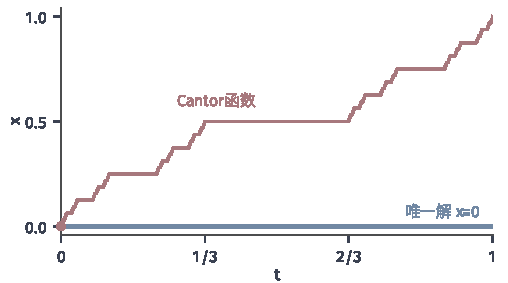
\includegraphics[width=86mm]{figures/06-differential-equations/01-ordinary-differential-equations/matplotlib/odeex-cantor-false/figure.pdf}
  \caption{绝对连续的必要性。方程是$\dot x=0$，$x(0)=0$，蓝线是它的唯一解$x\equiv0$。红线是Cantor函数，连续并几乎处处导数为零，但不绝对连续，不满足积分方程，因而不算解。}
  \label{fig:odeex-cantor-false}
\end{BookInlineFigure}

\paragraph{沿曲线的可测性}
积分方程要有意义，$s\mapsto\bm{f}(s,\bm{y}(s))$必须可测。条件只分别给出了对时间的可测性和对状态的连续性，下面的引理把两者合起来。

\begin{lemma}[沿连续曲线的可测性]
\label{lem:odeex-composition-measurable}
设$\bm{f}$满足定义~\ref{def:odeex-caratheodory}，$J'\subseteq J$是紧区间，$\bm{y}:J'\to\bm{C}$连续，$\bm{C}\subseteq\bm{\Omega}$紧。则$s\mapsto\bm{f}(s,\bm{y}(s))$在$J'$上可测，且可积。
\end{lemma}

\begin{proof}
把$J'$等分为$2^j$段，令$\bm{y}_j$在每段上取$\bm{y}$在该段左端点的值，右端点处取$\bm{y}$的值。在每段上$\bm{y}_j$是常向量，由条件1，$s\mapsto\bm{f}(s,\bm{y}_j(s))$在每段上可测，从而在$J'$上可测。

$\bm{y}$连续，所以$\bm{y}_j(s)\to\bm{y}(s)$对每个$s$成立。由条件2，对几乎每个$s$，$\bm{f}(s,\bm{y}_j(s))\to\bm{f}(s,\bm{y}(s))$。可测函数列的几乎处处极限可测，所以$\bm{f}(s,\bm{y}(s))$可测。可积性由式~\eqref{eq:odeex-caratheodory-bound}得到。
\end{proof}

\paragraph{局部存在}
Euler折线在这里不能用了。Euler格式需要右端在网格时刻$t_k$的值，而可测函数在单点的值没有意义，改变零测集上的值不改变方程，却能任意改变Euler格式。

替代办法是Tonelli的延迟逼近：用稍早一段的已知曲线计算积分，这样积分号里永远只含已经算好的部分，不需要逐点取值。

\begin{theorem}[Carathéodory存在定理]
\label{thm:odeex-caratheodory-existence}
设$\bm{f}$满足定义~\ref{def:odeex-caratheodory}，$[t_0,t_0+a]\subseteq J$，$\bm{B}_b\subseteq\bm{\Omega}$，$m\in L^1([t_0,t_0+a])$是$\bm{C}=\bm{B}_b$上的式~\eqref{eq:odeex-caratheodory-bound}的上界。取$\delta\in(0,a]$，使
\begin{equation}
 \int_{t_0}^{t_0+\delta}m(s)\,\mathrm{d}s\leq b.
 \label{eq:odeex-caratheodory-window}
\end{equation}
则初值问题在$[t_0,t_0+\delta]$上有取值于$\bm{B}_b$的Carathéodory解。$t_0$左侧有对称的结论。
\end{theorem}

积分$\int_{t_0}^{t_0+\delta}m$在$\delta\to0$时趋于零，满足式~\eqref{eq:odeex-caratheodory-window}的$\delta$总存在。它是$\delta\leq b/M$的自然推广：盒子的高度$b$现在由累计的速度上限来消耗。

\begin{proof}
\emph{延迟逼近。}记$I^+=[t_0,t_0+\delta]$，对正整数$N$，记$r=\delta/N$。定义$\bm{y}_N$：在$[t_0,t_0+r]$上$\bm{y}_N\equiv\bm{x}_0$；对$t\in(t_0+r,t_0+\delta]$，
\[
 \bm{y}_N(t)=\bm{x}_0+\int_{t_0}^{t-r}\bm{f}(s,\bm{y}_N(s))\,\mathrm{d}s.
\]
这个定义逐段进行：$t$在第$j+1$段时，积分只用到前$j$段上已定义的$\bm{y}_N$。由引理~\ref{lem:odeex-composition-measurable}，积分有定义。由式~\eqref{eq:odeex-caratheodory-window}，
\[
 \lVert\bm{y}_N(t)-\bm{x}_0\rVert_2\leq\int_{t_0}^{t-r}m(s)\,\mathrm{d}s\leq b,
\]
所以$\bm{y}_N$的取值都在$\bm{B}_b$中，递推能够继续。

\emph{等度连续。}令$W(\rho)$为$m$在$I^+$中长度不超过$\rho$的区间上积分的最大值。Lebesgue积分的绝对连续性给出$\rho\to0$时$W(\rho)\to0$。对$s<t$，$\bm{y}_N(t)-\bm{y}_N(s)$是一段长度不超过$t-s$的区间上的积分（或为零），所以
\[
 \lVert\bm{y}_N(t)-\bm{y}_N(s)\rVert_2\leq W(t-s).
\]
界$W$对所有$N$相同，$\{\bm{y}_N\}$一致有界且等度连续。由Arzelà--Ascoli判据，存在子列在$I^+$上一致收敛到连续曲线$\bm{x}:I^+\to\bm{B}_b$。

\emph{取极限。}把延迟积分写成到$t$的积分减去尾部，对所有$t\in I^+$（$t<t_0+r$时也成立）有
\[
 \bm{y}_N(t)=\bm{x}_0+\int_{t_0}^{t}\bm{f}(s,\bm{y}_N(s))\,\mathrm{d}s-\bm{E}_N(t),\qquad
 \lVert\bm{E}_N(t)\rVert_2\leq W(r).
\]
沿子列，$\bm{y}_N(s)\to\bm{x}(s)$，由条件2，对几乎每个$s$，$\bm{f}(s,\bm{y}_N(s))\to\bm{f}(s,\bm{x}(s))$。被积函数以$m$为可积控制，由控制收敛定理，积分收敛。尾部$\bm{E}_N$趋于零。

令$N\to\infty$，$\bm{x}$满足积分方程~\eqref{eq:odeex-integral}，因而是Carathéodory解。左侧用时间反演$s\mapsto2t_0-s$得到。
\end{proof}

图~\ref{fig:odeex-tonelli-delay}对切换输入的例子画出了延迟逼近。开头的一段$r$内曲线不动，因为积分尚未开始；之后曲线滞后真解一段时间，$N$增大时滞后变短，逐渐贴合真解。

\begin{BookInlineFigure}
  \centering
  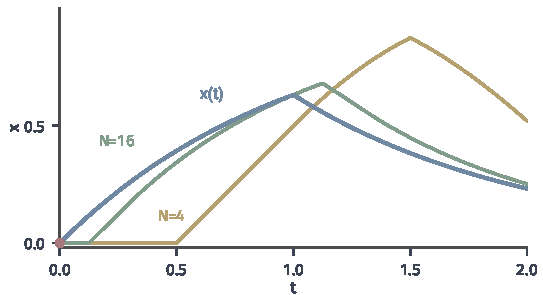
\includegraphics[width=92mm]{figures/06-differential-equations/01-ordinary-differential-equations/matplotlib/odeex-tonelli-delay/figure.pdf}
  \caption{延迟逼近。方程是$\dot x=-x+g(t)$，$x(0)=0$，$g$是图~\ref{fig:odeex-measurable-switch}(a)的切换输入，$\delta=2$。蓝线是解，黄线和绿线是$N=4$和$N=16$的延迟逼近$y_N$，延迟长度$r=\delta/N$。}
  \label{fig:odeex-tonelli-delay}
\end{BookInlineFigure}

\paragraph{唯一性}
存在定理对状态只要求连续，唯一性仍要另外的条件。第~\ref{sec:odeex-uniqueness}节的最后一个反例说明，对时间不一致的Lipschitz常数可以破坏唯一性；但$L$不必有界，可以放宽到$L$随时间局部可积。

\begin{theorem}[可积Lipschitz系数下的唯一性]
\label{thm:odeex-caratheodory-unique}
在定理~\ref{thm:odeex-caratheodory-existence}的记号下，设存在$\ell\in L^1([t_0,t_0+a])$，使对几乎每个$t\in[t_0,t_0+a]$和所有$\bm{x},\bm{y}\in\bm{B}_b$，
\begin{equation}
 \lVert\bm{f}(t,\bm{x})-\bm{f}(t,\bm{y})\rVert_2\leq\ell(t)\lVert\bm{x}-\bm{y}\rVert_2.
 \label{eq:odeex-integrable-lipschitz}
\end{equation}
取$\delta\in(0,a]$满足式~\eqref{eq:odeex-caratheodory-window}，以及
\begin{equation}
 \int_{t_0}^{t_0+\delta}\ell(s)\,\mathrm{d}s\leq\frac12.
 \label{eq:odeex-integrable-window}
\end{equation}
则初值问题在$[t_0,t_0+\delta]$上恰有一个取值于$\bm{B}_b$的Carathéodory解，Picard迭代~\eqref{eq:odeex-picard-iteration}一致收敛到它，并满足式~\eqref{eq:odeex-picard-error}。
\end{theorem}

\begin{proof}
证明与定理~\ref{thm:odeex-picard-lindelof}逐步对应。令$\mathcal{X}$为$[t_0,t_0+\delta]$上取值于$\bm{B}_b$的连续曲线组成的集合，它在一致距离下完备。

对$\bm{u}\in\mathcal{X}$，由引理~\ref{lem:odeex-composition-measurable}，$\mathcal{T}\bm{u}$有定义且连续，由式~\eqref{eq:odeex-caratheodory-window}，其取值在$\bm{B}_b$中。对$\bm{u},\bm{v}\in\mathcal{X}$，由式~\eqref{eq:odeex-integrable-lipschitz}和式~\eqref{eq:odeex-integrable-window}，
\[
 \lVert\mathcal{T}\bm{u}-\mathcal{T}\bm{v}\rVert_{\infty}
 \leq\int_{t_0}^{t_0+\delta}\ell(s)\lVert\bm{u}(s)-\bm{v}(s)\rVert_2\,\mathrm{d}s
 \leq\frac12\lVert\bm{u}-\bm{v}\rVert_{\infty}.
\]
由压缩映射定理得到唯一的不动点，它满足积分方程。取值于$\bm{B}_b$的Carathéodory解都是$\mathcal{T}$的不动点，所以都等于它。
\end{proof}

这里的压缩常数不再是“$L$乘时间”，而是系数的累计量$\int\ell$，后者由积分的绝对连续性保证在短时间内很小。一个解若从$\bm{x}_0$出发，由连续性在一小段时间内留在$\bm{B}_b$中，所以两条解在初始时刻重合后，局部总是相同的。

\begin{example}[系数无界的唯一性]
\label{ex:odeex-integrable-lipschitz}
考虑$\dot x=x/(2\sqrt{t})$，$x(0)=1$，取$b=1$。在$\lvert x-1\rvert\leq1$上，上界和Lipschitz系数分别可取
\[
 m(t)=\frac{1}{\sqrt{t}},\qquad\ell(t)=\frac{1}{2\sqrt{t}}.
\]
两者在$t\to0$时无界，但都可积。由$\int_0^\delta m=2\sqrt{\delta}$和$\int_0^\delta\ell=\sqrt{\delta}$，取$\delta=1/4$，式~\eqref{eq:odeex-caratheodory-window}和式~\eqref{eq:odeex-integrable-window}都成立。

从$x^{(0)}=1$出发迭代，第一步对$1/(2\sqrt{s})$积分，第二步对$(1+\sqrt{s})/(2\sqrt{s})$积分，分别得到
\[
 x^{(1)}=1+\sqrt{t},\qquad x^{(2)}=1+\sqrt{t}+\frac{t}{2}.
\]

一般地，$x^{(k)}=\sum_{j=0}^{k}(\sqrt{t})^j/j!$，极限是$\mathrm{e}^{\sqrt{t}}$。在$t=1/4$处，三轮迭代的取值依次是
\[
 1.5,\quad1.625,\quad1.6458,
\]
真解是$\mathrm{e}^{1/2}\approx1.6487$。
\end{example}

图~\ref{fig:odeex-integrable-lipschitz}比较了这个例子的系数与方程~\eqref{eq:odeex-clip}的系数。$1/(2\sqrt{t})$虽然也在原点无界，但其下的面积有限，短时间窗内的累计量可以小于$1/2$；$2/t$在原点附近的面积发散，没有任何时间窗能让累计量变小，多解正是从这里产生的。

\begin{BookInlineFigure}
  \centering
  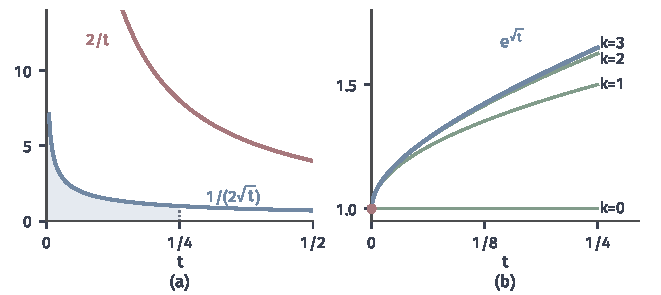
\includegraphics[width=112mm]{figures/06-differential-equations/01-ordinary-differential-equations/matplotlib/odeex-integrable-lipschitz/figure.pdf}
  \caption{时间上的Lipschitz系数。(a)蓝线$1/(2\sqrt{t})$可积，浅蓝面积是$[0,1/4]$上的累计量$1/2$；红线$2/t$在原点不可积。(b)$\dot x=x/(2\sqrt{t})$，$x(0)=1$的Picard迭代$x^{(0)},\ldots,x^{(3)}$（绿线）和解$\mathrm{e}^{\sqrt{t}}$（蓝线）。}
  \label{fig:odeex-integrable-lipschitz}
\end{BookInlineFigure}

\paragraph{唯一性不来自可测性或增长控制}
方程~\eqref{eq:odeex-sqrt}的右端满足Carathéodory条件，局部有界，并且至多线性增长，定理~\ref{thm:odeex-caratheodory-existence}保证它有解，但它有无穷多个解。时间可测性是对时间方向的放宽，增长控制处理的是解走多远，两者都不涉及两条解在状态方向上是否分开。方程~\eqref{eq:odeex-clip}也满足Carathéodory条件，它失败的原因是系数$2/t$不局部可积。

\paragraph{延拓与全局存在}
第~\ref{sec:odeex-maximal}节和第~\ref{sec:odeex-global}节的论证只用到积分方程，以及局部定理的时间窗在紧集上有统一下限，因此在下述条件下可以照搬：$\bm{f}$满足定义~\ref{def:odeex-caratheodory}，并且对每个紧区间$J'\subseteq J$和紧集$\bm{C}\subseteq\bm{\Omega}$，存在$\ell\in L^1(J')$，使式~\eqref{eq:odeex-integrable-lipschitz}在$J'\times\bm{C}$上成立。

唯一改动的地方是时间窗的选取。设$J$开，$\bm{K}\subseteq J\times\bm{\Omega}$紧，按引理~\ref{lem:odeex-uniform-window}的方式把$\bm{K}$放大成紧集，其上有共同的$m,\ell$。积分的绝对连续性给出一个$\delta_{\bm{K}}>0$，使$m$和$\ell$在任何长度不超过$\delta_{\bm{K}}$的时间段上的积分分别不超过$\rho/2$和$1/2$。

于是最大绝对连续解存在且唯一，最大存在区间在$J$中相对开，有限端点处解离开每个紧集。若增长条件~\eqref{eq:odeex-linear-growth}对几乎每个$t$成立，系数$\alpha,\beta$局部可积，定理~\ref{thm:odeex-global}及其上界~\eqref{eq:odeex-global-bound}也成立，因为那里的证明本来就只用了积分方程。切换输入的线性方程就属于这种情形，其解在整个时间轴上存在。

\section{流形上的局部解}
\label{sec:odeex-manifold}

球面上的风场、圆周上的匀速转动都是流形上的方程：未知量是流形上的一条曲线，右端是每点的切向量。流形没有全局的坐标，不能直接把上面的定理搬过去。办法是分两步：在一张坐标图内，方程就是欧氏空间的初值问题；跨图时，再用唯一性保证各张图上解出来的是同一条曲线。

\paragraph{坐标中的方程}
本节$M$是$n$维无边界光滑流形，$X$是$M$上的光滑向量场，流形、切向量与向量场的定义可参考\BookChapterRef{chap:manifold-basics}{卷四第24章“流形的基本概念”}。若可微曲线$\gamma:I\to M$对所有$t\in I$满足
\begin{equation}
 \dot\gamma(t)=X_{\gamma(t)},
 \label{eq:odeex-integral-curve}
\end{equation}
就称$\gamma$是$X$的\term{积分曲线}（integral curve）。

取坐标图$(U,\varphi)$，$X$在$U$上写成$X=\sum_iX_i\partial_i$。把分量读成坐标的函数，记
\[
 \bm{F}(\bm{x})=\bigl(X_1(\varphi^{-1}(\bm{x})),\ldots,X_n(\varphi^{-1}(\bm{x}))\bigr),\qquad\bm{x}\in\varphi(U).
\]
曲线的坐标记录$\bm{x}(t)=\varphi(\gamma(t))$的速度分量就是$\dot{\bm{x}}$，所以在$U$内，方程~\eqref{eq:odeex-integral-curve}等价于
\begin{equation}
 \dot{\bm{x}}=\bm{F}(\bm{x}).
 \label{eq:odeex-chart-equation}
\end{equation}
这是开集$\varphi(U)\subseteq\mathbb{R}^{n}$上的自治方程，右端光滑，第~\ref{sec:odeex-uniqueness}节的定理可用。

换一张图$(V,\psi)$，转移映射是$\tau=\psi\circ\varphi^{-1}$，同一条曲线的新记录是$\bm{y}=\tau(\bm{x})$。由链式法则，
\[
 \dot{\bm{y}}=\bm{J}_\tau(\bm{x})\dot{\bm{x}}=\bm{J}_\tau(\bm{x})\bm{F}(\bm{x}).
\]
切向量的分量按Jacobian矩阵变换，右端正好是$X$在新图中的分量$\bm{G}(\bm{y})$。因此$\bm{y}$满足新图中的方程$\dot{\bm{y}}=\bm{G}(\bm{y})$，两张图说的是同一件事，如图~\ref{fig:odeex-chart-transfer}。

\begin{BookInlineFigure}
  \centering
  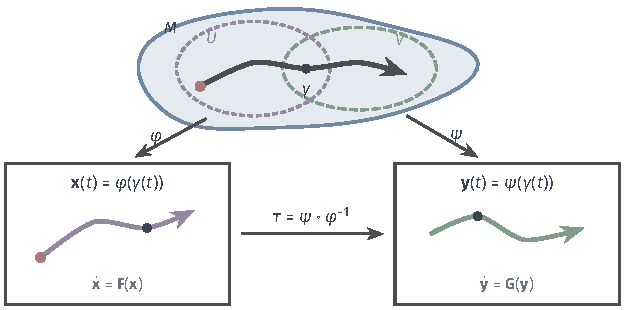
\includegraphics[width=106mm]{figures/06-differential-equations/01-ordinary-differential-equations/tikz/odeex-chart-transfer/figure.pdf}
  \caption{流形上的同一条积分曲线在两张坐标图中的记录。深灰曲线是$M$上的$\gamma$，紫色虚线和绿色虚线围成图的定义域$U,V$，下方是对应的坐标平面，曲线$\bm{x}$与$\bm{y}$分别满足各自的坐标方程。在重叠部分，黑点是同一个状态，转移映射$\tau$把一个方程变成另一个。}
  \label{fig:odeex-chart-transfer}
\end{BookInlineFigure}

\paragraph{局部解的拼接}
现在把第~\ref{sec:odeex-maximal}节的结论逐条搬到流形上。证明的结构不变，只是“盒子”换成坐标图内的盒子，距离的比较只在一张图内进行。

\begin{theorem}[积分曲线]
\label{thm:odeex-manifold}
设$M$是$n$维无边界光滑流形，$X$是其上的光滑向量场。
\begin{enumerate}
 \item 对每个$p\in M$，存在$\varepsilon>0$和积分曲线$\gamma:(-\varepsilon,\varepsilon)\to M$，使$\gamma(0)=p$。
 \item 若两条积分曲线定义在同一区间$I$上，且在某时刻取值相同，则它们在$I$上相同。
 \item 对每个$p\in M$，存在唯一的\term{最大积分曲线}（maximal integral curve）$\gamma_p:I_p\to M$，$\gamma_p(0)=p$，$I_p$是含$0$的开区间，以$p$为起点的积分曲线都是它的限制。
 \item 若$\omega_+=\sup I_p<+\infty$，则对$M$的每个紧子集$C$，存在$t_C\in I_p$，使当$t\in(t_C,\omega_+)$时$\gamma_p(t)\notin C$。
 \item 若$M$紧，则$I_p=\mathbb{R}$对每个$p$成立。
\end{enumerate}
\end{theorem}

\begin{proof}
\emph{结论1。}取含$p$的坐标图，在式~\eqref{eq:odeex-chart-equation}上应用定理~\ref{thm:odeex-picard-lindelof}，得到取值于$\varphi(U)$的解$\bm{x}$，令$\gamma=\varphi^{-1}\circ\bm{x}$。

\emph{结论2。}令$S=\{t\in I:\gamma_1(t)=\gamma_2(t)\}$，它非空。$M$是Hausdorff空间，$M\times M$的对角线闭，映射$t\mapsto(\gamma_1(t),\gamma_2(t))$连续，所以$S$在$I$中闭。

任取$t^\ast\in S$，取含$\gamma_1(t^\ast)$的坐标图$(U,\varphi)$。由连续性，$t^\ast$的某个邻域内两条曲线都留在$U$中，它们的坐标记录都解方程~\eqref{eq:odeex-chart-equation}并在$t^\ast$取相同的值，由定理~\ref{thm:odeex-picard-lindelof}重合。所以$S$在$I$中开，由连通性，$S=I$。

\emph{结论3。}与定理~\ref{thm:odeex-maximal}的证明相同：结论2使所有以$p$为起点的积分曲线相容，它们的并是最大积分曲线；若右端点属于$I_p$，从该点解局部问题就能再延长一段。

\emph{结论4。}先选有限覆盖。对每点$q\in C$取含它的坐标图及其内的一个紧邻域，$C$紧，所以有限个紧邻域$C_1,\ldots,C_r$覆盖$C$，各含于坐标图$(U_i,\varphi_i)$。对紧集$\{0\}\times\varphi_i(C_i)$应用引理~\ref{lem:odeex-uniform-window}，得到时间窗$\delta_i$，令$\delta=\min_i\delta_i$。从$C$的任一点出发的积分曲线至少存在时间$\delta$。

反设存在$t_j\uparrow\omega_+$使$\gamma_p(t_j)\in C$，取$j$使$t_j+\delta>\omega_+$。$X$不显含时间，所以从$\gamma_p(t_j)$出发、再走时间$\delta$的积分曲线平移后接在$\gamma_p$之后，由结论2相容，它越过了$\omega_+$，矛盾。

\emph{结论5。}取$C=M$，$\gamma_p(t)$不可能离开$M$，由结论4，$\sup I_p=+\infty$；对$-X$同样推理，$\inf I_p=-\infty$。
\end{proof}

结论2用到了流形定义中的Hausdorff条件，局部的Picard定理本身用不上它。在双原点直线上取向量场$\partial_x$，从$x=-1$出发的积分曲线到$t=1$时可以到达任一个原点：两条积分曲线在$t<1$时重合，在$t=1$时不同，局部唯一性并不能排除这一点。流形的定义排除了这种空间。满足结论5的向量场称为\term{完备向量场}（complete vector field）。

\paragraph{图内爆炸不是流形上爆炸}
定理~\ref{thm:odeex-escape}用在坐标方程上时，说的是解离开$\varphi(U)$的紧子集，这可能只是走出了这张图。单位圆$S^1$上的匀速转动是最简单的例子。

设$\bm{y}=(\sin\alpha,-\cos\alpha)$，$\alpha=0$是南极，$\alpha=\pi$是北极。令向量场使$\dot\alpha=2$。取从北极出发的球极投影作图：$u=y_1/(1-y_2)$，定义域是$S^1$去掉北极，代入得到$u=\tan(\alpha/2)$。求导，$X$在这张图中的方程是
\[
 \dot u=\frac{1}{2\cos^2(\alpha/2)}\dot\alpha=1+u^2.
\]

从南极出发，$u(0)=0$，解是$u=\tan t$，在$t=\pi/2$时趋于无穷。这与$\dot x=1+x^2$的爆炸是同一个公式，但这里的$u\to\infty$只意味着曲线走向北极，也就是走出了这张图。

换用从南极出发的投影$v=y_1/(1+y_2)$，定义域是$S^1$去掉南极。转移映射是$v=1/u$，所以新图中的方程为
\[
 \dot v=-\frac{\dot u}{u^2}=-\frac{1+u^2}{u^2}=-(1+v^2).
\]
在$t=\pi/4$时，$u=1$，$v=1$。从这里在第二张图中继续解，得到$v=\cot t$，它在$t=\pi/2$时取值$0$，平稳地经过北极。图~\ref{fig:odeex-chart-blowup}显示了这次换图。

\begin{BookInlineFigure}
  \centering
  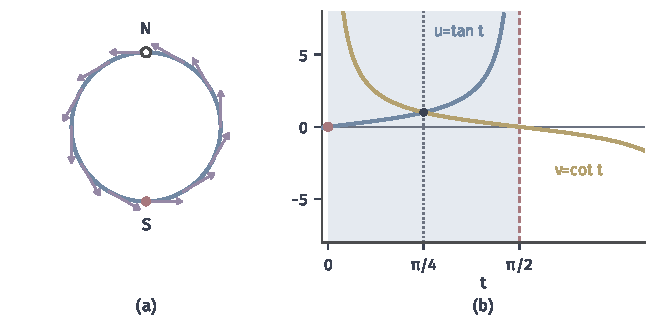
\includegraphics[width=112mm]{figures/06-differential-equations/01-ordinary-differential-equations/matplotlib/odeex-chart-blowup/figure.pdf}
  \caption{图内爆炸不是流形上爆炸。(a)单位圆上的匀速旋转场（紫色箭头），红点是南极$S$，空心点是第一张图未覆盖的北极$N$。(b)蓝线是第一张图的坐标$u=\tan t$，在红色虚线$t=\pi/2$爆炸；黄线是第二张图的坐标$v=\cot t$，在该处取值$0$。黑点是$t=\pi/4$处的换图点，$u=v=1$。}
  \label{fig:odeex-chart-blowup}
\end{BookInlineFigure}

圆是紧流形，由定理~\ref{thm:odeex-manifold}的结论5，积分曲线对所有$t$存在，这里$\alpha=2t$确实如此。

\paragraph{嵌入流形上的切向量场}
流形常常作为$\mathbb{R}^{N}$中的约束集合出现。设$M\subseteq\mathbb{R}^{N}$是嵌入子流形，$W\supseteq M$是开集，$\tilde{\bm{f}}:W\to\mathbb{R}^{N}$光滑，并且在$M$上切于$M$，即$\tilde{\bm{f}}(\bm{p})\in T_{\bm{p}}M$。我们希望知道，从$M$上出发解环境方程$\dot{\bm{y}}=\tilde{\bm{f}}(\bm{y})$，解是否留在$M$上。

唯一性给出的回答很简洁。$\tilde{\bm{f}}$限制在$M$上是$M$的向量场，由定理~\ref{thm:odeex-manifold}有$M$内的积分曲线$\gamma$。把$\gamma$看成$\mathbb{R}^{N}$中的曲线，它就是环境方程的解。环境方程的解是唯一的，所以环境解在$\gamma$存在的时间段内就是$\gamma$，它留在$M$上。约束不需要在算法上另外施加，切向条件加唯一性就够了。

\begin{example}[球面上的旋转场]
\label{ex:odeex-sphere-rotation}
在$\mathbb{R}^{3}$中取$\tilde{\bm{f}}(\bm{y})=(-y_2,y_1,0)$。对$\bm{y}\in S^2$，有$\langle\bm{y},\tilde{\bm{f}}(\bm{y})\rangle=0$，场切于球面。环境方程是线性的，解为绕竖直轴的旋转，保持$\lVert\bm{y}\rVert_2=1$。把$\tilde{\bm{f}}$换成不切的场$(1,0,0)$，解$\bm{y}_0+t(1,0,0)$立即离开球面。
\end{example}

\paragraph{测地线的初值问题}
黎曼流形$(M,g)$上的测地线方程在坐标中写作
\begin{equation}
 \ddot x_k+\sum_{i,j}\Gamma^k_{i,j}(\bm{x})\,\dot x_i\dot x_j=0,\qquad k=1,\ldots,n.
 \label{eq:odeex-geodesic}
\end{equation}
相关的定义可参考\BookChapterRef{chap:riemannian-geometry}{卷四第27章“黎曼几何”}。那里陈述并使用了光滑方程的局部理论，局部存在唯一、最大解和离开紧集三项在这一节得到了证明，光滑依赖由第~\ref{chap:ode-sensitivity}章证明。

它是二阶方程，状态要包括位置和速度。令$\bm{w}=\dot{\bm{x}}$，得到一阶系统
\[
 \dot{\bm{x}}=\bm{w},\qquad\dot w_k=-\sum_{i,j}\Gamma^k_{i,j}(\bm{x})\,w_iw_j.
\]
右端在$\varphi(U)\times\mathbb{R}^{n}$上光滑，定理~\ref{thm:odeex-picard-lindelof}给出局部解。全体$(p,\bm{w})$（$p\in M$，$\bm{w}\in T_pM$）组成的集合称为\term{切丛}（tangent bundle），记为$TM$，它是$2n$维流形，$(\bm{x},\bm{w})$是其坐标。

测地线就是$TM$上一个向量场的积分曲线在$M$上的投影。条件$D\dot\gamma/\mathrm{d}t=0$不依赖坐标，所以不同的图给出的是同一条曲线，定理~\ref{thm:odeex-manifold}的结论都适用：每个初始位置和初始速度决定唯一的最大测地线。

速度的长度沿测地线不变，这给出了$M$紧时的整体结论。设$M$紧，$\lVert\dot\gamma\rVert_g$恒等于初始速度的长度$c$，于是$(\gamma,\dot\gamma)$始终留在集合$\{(p,\bm{w})\in TM:g_p(\bm{w},\bm{w})=c^2\}$中，这个集合是紧的。由结论4，测地线对所有$t$存在。

球面上还可以把测地线写成环境方程，直接看约束是如何保持的。$S^2\subset\mathbb{R}^{3}$的测地线加速度沿法向，方程是
\begin{equation}
 \ddot{\bm{y}}=-\lVert\dot{\bm{y}}\rVert_2^2\,\bm{y}.
 \label{eq:odeex-sphere-geodesic}
\end{equation}
右端是$(\bm{y},\dot{\bm{y}})\in\mathbb{R}^{6}$的光滑函数，在$\mathbb{R}^{3}$中到处都有定义。设初值满足$\lVert\bm{y}(0)\rVert_2=1$和$\langle\bm{y}(0),\dot{\bm{y}}(0)\rangle=0$。

令$c=\lVert\bm{y}\rVert_2^2-1$，$d=\langle\bm{y},\dot{\bm{y}}\rangle$，它们衡量解偏离约束的程度。由式~\eqref{eq:odeex-sphere-geodesic}，
\[
 \dot c=2d,\qquad\dot d=\lVert\dot{\bm{y}}\rVert_2^2+\langle\bm{y},\ddot{\bm{y}}\rangle=-\lVert\dot{\bm{y}}\rVert_2^2\,c.
\]
沿给定的解，$\lVert\dot{\bm{y}}(t)\rVert_2^2$是已知的连续函数，这是关于$(c,d)$的线性系统，初值为零。由唯一性，$(c,d)\equiv\bm{0}$，解永远留在球面上，速度永远切于球面。

取$\bm{p}=(1,0,0)$，$\bm{v}=(0,1,0)$，解是赤道$\bm{y}(t)=(\cos t,\sin t,0)$，此时$\lVert\dot{\bm{y}}\rVert_2^2=1$，$\ddot{\bm{y}}=-\bm{y}$，方程成立。图~\ref{fig:odeex-sphere-constraint}(b)中的蓝线是数值积分得到的$\lVert\bm{y}\rVert_2^2-1$，保持为零。

若初速度不切于球面，例如$\bm{v}=(0.25,1,0)$，则$(c,d)$的初值不为零，$c$随时间偏离零，图中红线的最大值约为$0.39$。约束是否保持，完全取决于初值是否在约束集合上，这正是唯一性的结论。

\begin{BookInlineFigure}
  \centering
  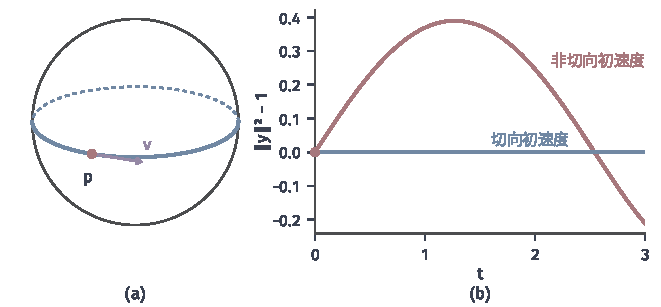
\includegraphics[width=112mm]{figures/06-differential-equations/01-ordinary-differential-equations/matplotlib/odeex-sphere-constraint/figure.pdf}
  \caption{球面测地线的环境方程~\eqref{eq:odeex-sphere-geodesic}。(a)单位球面上过红点$\bm{p}$、初速度为紫色箭头$\bm{v}$的测地线（赤道，背面用虚线）。(b)约束偏差$\lVert\bm{y}\rVert_2^2-1$：蓝线是切向初速度$(0,1,0)$，恒为零；红线是非切向初速度$(0.25,1,0)$，解离开球面。}
  \label{fig:odeex-sphere-constraint}
\end{BookInlineFigure}

平行移动方程
\[
 \dot V_k+\sum_{i,j}\Gamma^k_{i,j}(\bm{x}(t))\,\dot x_iV_j=0
\]
是关于$V$的线性方程，系数沿给定曲线连续。由例~\ref{ex:odeex-linear-global}，它在曲线的整个定义区间上有唯一解，跨图时由唯一性分段接续。测地线方程则是速度的二次方程，局部解未必能延伸到所有时间，这与开单位球上直线走到边界的情形一致，也正是定理~\ref{thm:odeex-escape}所说的状况。

\section{本章小结}
\label{sec:odeex-summary}

章首的三个方程分别暴露了三个问题：$\dot x=x^2$在有限时间内走不下去，$\dot x=2\sqrt{\lvert x\rvert}$有多条解，右端跳变的方程从零点出发无解。本章逐一给出了这些问题的条件，图~\ref{fig:odeex-summary-map}把它们串在一起。

局部存在只回答“有没有解”。有限维空间中右端连续就够了：Euler折线被关在盒子内，紧性抽出收敛的子列，连续性让极限满足方程。这条路线只给出一个解，子列的选择甚至依赖扰动，在无限维空间也可能失败。

唯一性回答“解是否由初值确定”。状态方向的局部Lipschitz条件使积分映射在短时间窗内成为压缩映射，靠完备性而不是紧性得到不动点，存在、唯一和迭代误差界同时得到。这一条件是便于验证的充分条件，单调性也能给出单向的唯一性；但Lipschitz常数对时间不局部可积时，唯一性可以失败。

\begin{BookInlineFigure}
  \centering
  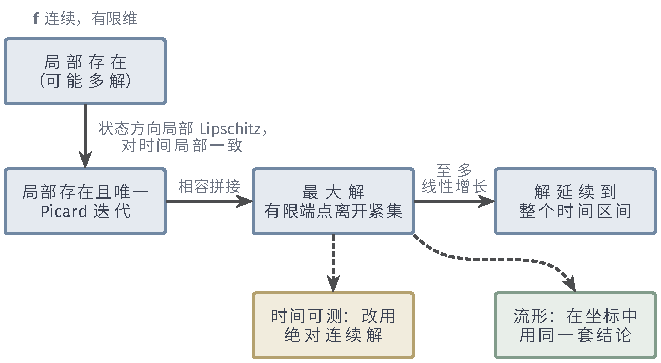
\includegraphics[width=112mm]{figures/06-differential-equations/01-ordinary-differential-equations/tikz/odeex-summary-map/figure.pdf}
  \caption{本章结论的依赖关系。从连续右端的局部存在出发，加上状态方向的局部Lipschitz条件得到局部存在且唯一，相容拼接得到最大解，至多线性增长使解延续到整个时间区间。虚线表示同一链条的两个推广：时间可测的方程和流形上的方程。}
  \label{fig:odeex-summary-map}
\end{BookInlineFigure}

最大延拓回答“局部解能接多长”。唯一性使局部解相容，并成唯一的最大解。解的定义区间是开区间，到有限端点时解离开定义域的每个紧集，表现为状态无界或趋近定义域的边界。全局存在回答“解能否走完给定的时间区间”，至多线性增长的右端保证了这一点，但解仍可能无界，全局存在也不提供唯一性。表~\ref{tab:odeex-summary}按问题列出了条件和反例。

\begin{BookInlineTable}
  \centering
  \caption{各问题的条件与反例}
  \label{tab:odeex-summary}
  \begin{tabularx}{\linewidth}{lXX}
    \toprule
    问题 & 条件（$\bm{f}$连续时） & 去掉条件的反例 \\
    \midrule
    局部存在 & 有限维，$\bm{f}$连续 & 右端跳变无解；$c_0$上连续而无解 \\
    唯一性 & 状态方向局部Lipschitz，对时间局部一致 & $2\sqrt{\lvert x\rvert}$的漏斗；系数$2/t$ \\
    最大延拓 & 局部存在且唯一 & 没有唯一性时最大解不唯一 \\
    全局存在 & 至多线性增长 & $\dot x=x^2$在$t=1$爆炸 \\
    \bottomrule
  \end{tabularx}
\end{BookInlineTable}

时间可测时，解要换成绝对连续解，对应的条件是：对时间可测、对状态连续、局部可积上界，由此得到存在；唯一性另要求状态方向的Lipschitz系数对时间局部可积，这不能由可测性或增长控制推出。这些结论只针对满足积分方程的绝对连续曲线，连续且几乎处处满足方程还不够，Cantor函数就是反例。

流形上，局部存在唯一性在每张坐标图内应用，切向量的变换规律使不同的图描述同一条曲线，Hausdorff条件和唯一性把它们接成最大积分曲线。坐标方程的爆炸可能只是走出了一张图，紧流形上的积分曲线对所有时间存在。切向条件和唯一性共同使解保持在流形上，测地线方程是这一结构的代表。

这些结论都只说明解的存在、唯一和存在区间，是有限时间上的定性结论。解对初值和参数怎样变化，变化能否求导，由第~\ref{chap:ode-sensitivity}章在这里的存在性保证上继续建立；第~\ref{chap:ode-numerical-methods}章的数值方法也是在解存在且唯一时才有明确的逼近目标。

